\documentclass[12pt, a4paper]{article}

% =====================================================================
%  Package/package.tex  -  PACKAGE DÙNG CHUNG (nạp 1 lần duy nhất)
%  Quy ước:
%   - Package dùng cho >= 2 chapter (hoặc main.tex) đặt ở file này.
%   - Package/cấu hình chỉ 1 chapter dùng đặt ở Package/Chapter_N/package.tex.
%   - Không \usepackage lại package chung trong file của chapter.
% =====================================================================

% ---------- Ngôn ngữ & mã hoá (thay cho vietnam + inputenc/fontenc rải rác) ----------
\usepackage[T5]{fontenc}
\usepackage[utf8]{inputenc}
\usepackage[vietnamese]{babel}

% ---------- Bố cục trang: canh lề cấu hình 1 chỗ duy nhất ----------
% (a4paper đã khai báo ở \documentclass nên không lặp lại)
\usepackage[margin=2cm]{geometry}

% ---------- Hình ảnh, màu, TikZ ----------
\usepackage{graphicx}             % Ch3, Ch4, Ch5, main (logo)
\usepackage{xcolor}               % màu listings (Ch3, Ch4, Ch5), TikZ
\usepackage{tikz}                 % main.tex (viền trang bìa)
\usetikzlibrary{calc}

% ---------- Toán ----------
\usepackage{amsmath, amssymb}     % Ch2, Ch3, Ch5

% ---------- Hình/bảng nổi, danh sách, giãn đoạn ----------
\usepackage{float}                % [H]: Ch1, Ch4, Ch5
\usepackage{enumitem}             % Ch2 (label=, leftmargin=*) + định dạng itemize/enumerate toàn bài
\setlist[itemize]{label=-, topsep=4pt, itemsep=3pt}
\setlist[enumerate]{topsep=4pt, itemsep=3pt}
\usepackage{parskip}              % giãn đoạn toàn bài (parindent = 0)

% ---------- Mã nguồn (listings): 1 định dạng chuẩn cho TOÀN BỘ chapter ----------
\usepackage{listings}
\definecolor{mybackground}{HTML}{FFFFFF}
\definecolor{mykeyword}{HTML}{000000}
\definecolor{mystring}{HTML}{990099}
\definecolor{mycomment}{HTML}{008000}

% Style nền: đặt lại mọi thuộc tính về giá trị xác định
\lstdefinestyle{lstbase}{
    language={},
    basicstyle=\ttfamily\small,
    keywordstyle=\bfseries,
    commentstyle=\itshape,
    stringstyle={},
    numbers=none,
    numberstyle=\tiny,
    stepnumber=1,
    numbersep=10pt,
    backgroundcolor={},
    frame=single,
    rulecolor={},
    xleftmargin=0pt,
    xrightmargin=0pt,
    framexleftmargin=0pt,
    aboveskip=\medskipamount,
    belowskip=\medskipamount,
    columns=fullflexible,   % giữ hiệu lực thực tế trước đây; copy code từ PDF không bị tách ký tự
    keepspaces=true,
    breaklines=true,
    breakatwhitespace=false,
    showspaces=false,
    showtabs=false,
    showstringspaces=false,
    tabsize=2,
    captionpos=t,
    escapeinside={}{}
}

% Style chuẩn dùng cho mọi \begin{lstlisting} (Ch3, Ch4, Ch5, ...)
\lstdefinestyle{lstmain}{
    style=lstbase,
    language=R,
    backgroundcolor=\color{mybackground},
    basicstyle=\ttfamily\small\color{black},
    keywordstyle=\color{mykeyword}\bfseries,
    stringstyle=\color{mystring},
    commentstyle=\color{mycomment}\itshape,
    numbers=left,
    numberstyle=\tiny\color{gray},
    stepnumber=1,
    numbersep=10pt,
    showspaces=false,
    showstringspaces=false,
    showtabs=false,
    frame=single,
    rulecolor=\color{black},
    tabsize=2,
    captionpos=b,
    breaklines=true,
    breakatwhitespace=false,
    escapeinside={\%*}{*)},
    xleftmargin=15pt,
    framexleftmargin=15pt
}
\lstset{style=lstmain}

% ---------- Tài liệu tham khảo ----------
\usepackage{csquotes}
\usepackage[backend=biber,style=ieee]{biblatex}
\addbibresource{reference/reference.bib}

% ---------- Package riêng của từng chapter ----------
% Chapter 1 - Tổng quan dữ liệu
% Dùng chung (đã nạp ở Package/package.tex): float [H], hyperref (\href), amsmath, enumitem
\usepackage{array}      % \newcolumntype, \arraybackslash
\usepackage{tabularx}   % bảng tabularx với cột Y, C tự định nghĩa trong chapter
\usepackage{ragged2e}   % \RaggedRight, \Centering

% Chapter 2 - Kiến thức nền
% Không cần package riêng. Dùng chung (nạp ở Package/package.tex):
%   amsmath (công thức), enumitem (itemize[label=..., leftmargin=*])

\usepackage{listings}
\usepackage{xcolor}
\usepackage{booktabs}
\usepackage{longtable}
\usepackage{float}
\lstset{
    language=C,
    basicstyle=\ttfamily\small,
    keywordstyle=\color{blue}\bfseries,
    commentstyle=\color{green!60!black},
    stringstyle=\color{red},
    showstringspaces=false,
    frame=single,
    numbers=left,
    numberstyle=\tiny\color{gray},
    breaklines=true,
    tabsize=4
}
\usepackage{parskip}
\usepackage{amsmath}
% Chapter 4 - Thống kê mô tả
% Không cần package riêng. Dùng chung (nạp ở Package/package.tex):
%   listings (style lstmain), xcolor, graphicx, float [H], enumitem

% Chapter 5 - Thống kê suy diễn
% Dùng chung (nạp ở Package/package.tex): amsmath, graphicx, float [H], listings (lstmain), xcolor, enumitem
\usepackage{setspace}
\onehalfspacing   % LƯU Ý: đặt ở preamble nên giãn dòng 1.5 áp dụng cho TOÀN BÀI (giữ nguyên như cũ)

% Khung hiển thị KẾT QUẢ R (dùng: \begin{lstlisting}[style=rout]); code R dùng style chuẩn lstmain ở root
\lstdefinestyle{rout}{
    language={},
    numbers=none,
    framexleftmargin=0pt,
    basicstyle=\ttfamily\scriptsize,
    breaklines=true,
    columns=fullflexible,
    keepspaces=true,
    frame=single,
    rulecolor=\color{black!30},
    backgroundcolor=\color{yellow!6},
    xleftmargin=0.3cm,
    xrightmargin=0.2cm,
    aboveskip=0.6em,
    belowskip=0.6em
}

% Chapter 6 - Thảo luận và mở rộng
% Chưa cần package riêng (dùng chung ở Package/package.tex).

% Chapter 7 - Nguồn dữ liệu và nguồn code
% Chưa cần package riêng (dùng chung ở Package/package.tex).


% ---------- hyperref: luôn nạp CUỐI CÙNG ----------
\usepackage{hyperref}
\hypersetup{
	colorlinks=true,
	linkcolor=black,
	urlcolor=blue
}

\geometry{a4paper, margin=2cm}


\begin{document}
	%Trang trí viền trang bìa
	\begin{tikzpicture}[remember picture,overlay]
            % Khung viền ngoài (nét đậm)
            \draw[blue!70!black, line width=3pt] 
                ([xshift=1.5cm, yshift=-1.5cm]current page.north west) 
                rectangle 
                ([xshift=-1.5cm, yshift=1.5cm]current page.south east);
            % Khung viền trong (nét mảnh)
            \draw[blue!70!black, line width=1pt] 
                ([xshift=1.65cm, yshift=-1.65cm]current page.north west) 
                rectangle 
                ([xshift=-1.65cm, yshift=1.65cm]current page.south east);
        \end{tikzpicture}
	
	%Trang 1 (trang bìa)
	\thispagestyle{empty}
	\begin{center}
		{
			\textbf{ĐẠI HỌC QUỐC GIA THÀNH PHỐ HỒ CHÍ MINH} \\ [3pt]
			\textbf{TRƯỜNG ĐẠI HỌC BÁCH KHOA} \\ [3pt]
			\textbf{KHOA KHOA HỌC ỨNG DỤNG} \\ [3pt]
		}
		\begin{tikzpicture}
			\draw[yshift=-0.3cm, dash pattern=on 3pt off 1pt] (0,0) -- (12,0);
		\end{tikzpicture}
	\end{center}
	
	\vspace{08pt}
	
	\begin{center}
		
\includegraphics[width=2.5in]{Image/logo}
	\end{center}
	
	\begin{center}
		{\Large \textbf{\MakeUppercase{BÁO CÁO BÀI TẬP LỚN}}} \\ 
		{\Large \textbf{\MakeUppercase{MÔN: XÁC SUẤT THỐNG KÊ (MT2013)}}} 
		\rule{16cm}{1pt} % Gạch chân dài 16cm, dày 1pt
		\\[10pt] % Khoảng cách giữa gạch chân và đề tài
		{\Large \textbf{\MakeUppercase{ĐỀ TÀI: \\PHÂN TÍCH PHÍ GIAO HÀNG\\ CỦA CỬA HÀNG BÁN LẺ}}}  %Tên đề tài
	\end{center}
	\begin{center}
		\rule{16cm}{1pt}
	\end{center}
	
	\vspace{1cm}
	
	\begin{center}
		\renewcommand{\arraystretch}{1.5}
        \begin{tabular}{rl}
            \Large \textbf{GVHD:} & \Large Nguyễn Bá Thi \\
            \Large \textbf{Lớp:} & \Large A01 \\
            \Large \textbf{Nhóm:} & \Large 12 \\
			\Large \textbf{KHOA:} & \Large Điện - Điện tử\\
        \end{tabular}
        
	\end{center}

	\vfill
	\begin{center}
		{\footnotesize Tp. Hồ Chí Minh, Tháng 12/2026}
	\end{center}
	\vspace{1cm}
	\pagebreak

\section*{Danh sách thành viên}

\vspace{1cm}

\begin{center}
    \renewcommand{\arraystretch}{1.5}
    \begin{tabularx}{\textwidth}{|c|X|c|c|X|}
        \hline
        \textbf{STT} & \textbf{Họ và tên thành viên} & \textbf{MSSV} & \textbf{\% Đóng góp} & \multicolumn{1}{c|}{\textbf{Điểm}} \\ \hline
        1 & Nguyễn Hoàng Anh & 2510421 & $100\%$ & \\ \hline
        2 & Nguyễn Minh Đức & 2510519 & $100\%$ & \\ \hline
        3 & Nguyễn Hải Dương & 2510532 & $100\%$ & \\ \hline
        4 & Đặng Hoàng Anh & 2510415 & $100\%$ & \\ \hline
        5 & Nguyễn Thái Dương & 2510534 & $100\%$ & \\ \hline
    \end{tabularx}
\end{center}

\section{Tổng quan dữ liệu}
adawdawwadawdwda

\section{Kiến thức nền}
	\subsection{Câu hỏi và mục tiêu nghiên cứu}	
	Nghiên cứu này tập trung vào việc ứng dụng hệ thống các phương pháp thống kê mô tả, thống kê suy diễn và mô hình hồi quy tuyến tính bội nhằm phân tích dữ liệu giao dịch của cửa hàng điện tử trực tuyến, từ đó khảo sát và dự báo Chi phí giao hàng (\texttt{delivery\_charges}). Trong đó nhóm đặt ra những câu hỏi sau:
	
	\begin{itemize}
		\item Các đặc trưng của đơn hàng và dịch vụ vận chuyển - bao gồm khoảng cách địa lý từ khách hàng đến kho hàng gần nhất, yêu cầu dịch vụ giao hàng nhanh, tổng giá trị đơn hàng, chính sách chiết khấu , vị trí kho xuất hàng, yếu tố mùa vụ  và mức độ hài lòng của khách hàng tác động theo chiều hướng và mức độ như thế nào đến chi phí giao hàng?
		\item Có sự khác biệt có ý nghĩa thống kê về chi phí vận chuyển hoặc giá trị đơn hàng giữa nhóm sử dụng dịch vụ giao hàng nhanh so với giao hàng tiêu chuẩn, cũng như giữa 4 mùa: Xuân, Hạ, Thu, Đông trong năm và giữa 3 khu vực kho hàng (\textit{Bakers}, \textit{Nickolson}, \textit{Thompson}) hay không?
		\item Mô hình hồi quy tuyến tính bội nào là tối ưu nhất sau khi sàng lọc biến để giải thích sự biến thiên và dự báo chính xác chi phí giao hàng cho các đơn hàng mới trong tương lai?
	\end{itemize}
	
	
	\subsection{Thống kê mô tả và Trực quan hóa dữ liệu}
	
	Trước khi thực hiện các suy diễn thống kê và xây dựng mô hình hồi quy, dữ liệu cần được làm sạch, kiểm tra công thức tính toán thực tế của tổng giá trị đơn hàng:
	\begin{equation}
		\text{\texttt{order\_total}} = \text{\texttt{order\_price}} \times \left(1 - \frac{\text{\texttt{coupon\_discount}}}{100}\right) + \text{\texttt{delivery\_charges}}
	\end{equation}
	và tóm tắt đặc trưng thông qua các đại lượng thống kê mô tả.
	
	\subsubsection{Các đại lượng thống kê mô tả mẫu}
	
	Giả sử có một mẫu ngẫu nhiên kích thước $n$ gồm các quan sát $x_1, x_2, \dots, x_n$ của một biến định lượng liên tục:
	
	\begin{itemize}
		\item Trung bình mẫu ($\bar{x}$): Đặc trưng cho xu hướng trung tâm của dữ liệu:
		\begin{equation}
			\bar{x} = \frac{1}{n} \sum_{i=1}^{n} x_i
		\end{equation}
		\item Trung vị mẫu ($Me$): Là giá trị nằm ở vị trí chính giữa của mẫu sau khi đã sắp xếp theo thứ tự không giảm $x_{(1)} \le x_{(2)} \le \dots \le x_{(n)}$:
		\begin{equation}
			Me = \begin{cases}
				x_{\left(\frac{n+1}{2}\right)} & \text{nếu } n \text{ lẻ}, \\[6pt]
				\dfrac{1}{2}\left(x_{\left(\frac{n}{2}\right)} + x_{\left(\frac{n}{2}+1\right)}\right) & \text{nếu } n \text{ chẵn}.
			\end{cases}
		\end{equation}
		\item Phương sai mẫu ($s^2$) và Độ lệch chuẩn mẫu ( $s$): Đo lường mức độ biến thiên và phân tán của các quan sát xung quanh trung bình mẫu:
		\begin{equation}
			s^2 = \frac{1}{n-1} \sum_{i=1}^{n} (x_i - \bar{x})^2, \qquad s = \sqrt{s^2}
		\end{equation}
		\item Khoảng tứ phân vị ($IQR$) và Quy tắc phát hiện ngoại lai:
		Các tứ phân vị $Q_1$, $Q_2$ và $Q_3$ chia mẫu đã sắp xếp thành 4 phần đều nhau. Khoảng tứ phân vị được xác định bởi:
		\begin{equation}
			IQR = Q_3 - Q_1
		\end{equation}
		Theo quy tắc rào chắn Tukey, một quan sát $x_i$ được nhận diện là giá trị ngoại lai cần được xử lý trong bước làm sạch dữ liệu nếu thỏa mãn:
		\begin{equation}
			x_i < Q_1 - 1.5 \times IQR \quad \text{hoặc} \quad x_i > Q_3 + 1.5 \times IQR
		\end{equation}
	\end{itemize}
	
	\subsubsection{Các công cụ trực quan hóa và Phân tích tương quan tuyến tính}
	
	\begin{itemize}
		\item Biểu đồ tần số: Biểu diễn phân phối thực nghiệm của các biến định lượng, giúp đánh giá tính đối xứng, độ lệch và sự tập trung của dữ liệu.
		\item Biểu đồ cột: Thể hiện bảng tần số của các biến phân loại, giúp so sánh quy mô đơn hàng giữa các danh mục.
		\item Biểu đồ hộp: Trực quan hóa 5 thông số ($\min, Q_1, Me, Q_3, \max$) của biến định lượng theo từng nhóm phân loại, hỗ trợ đối chiếu phân phối giữa các nhóm và phát hiện các điểm ngoại lai trước và sau khi làm sạch.
				\item Biểu đồ tương tác: Biểu diễn trung bình mẫu của biến định lượng theo từng tổ hợp của hai nhân tố phân loại và giúp quan sát trực quan xem các đường biểu diễn có song song hay cắt nhau, từ đó dự đoán sự tồn tại của hiệu ứng tương tác trước khi kiểm định bằng ANOVA.
		\item Biểu đồ phân tán và Hệ số tương quan mẫu Pearson ($r$): Để đánh giá mức độ liên kết tuyến tính giữa hai biến định lượng $X$ và $Y$ từ $n$ cặp quan sát $(x_i, y_i)$, hệ số tương quan mẫu Pearson được tính theo công thức:
		\begin{equation}
			r = \frac{\sum_{i=1}^{n} (x_i - \bar{x})(y_i - \bar{y})}{\sqrt{\sum_{i=1}^{n} (x_i - \bar{x})^2} \sqrt{\sum_{i=1}^{n} (y_i - \bar{y})^2}}, \qquad r \in [-1; 1]
		\end{equation}
		Để kiểm định xem hệ số tương quan tổng thể $\rho$ có thực sự khác 0 hay không ($H_0: \rho = 0$ đối với $H_1: \rho \neq 0$), ta sử dụng thống kê kiểm định $t$:
		\begin{equation}
			t_0 = \frac{r\sqrt{n - 2}}{\sqrt{1 - r^2}} \sim t(n - 2)
		\end{equation}
	\end{itemize}
	
	\subsection{Ước lượng khoảng tin cậy và Kiểm định giả thuyết hai mẫu}
	
	\subsubsection{Ước lượng khoảng tin cậy}
	
	Khoảng tin cậy với độ tin cậy $1 - \alpha$, thường chọn $1 - \alpha = 95\%$, ứng với mức ý nghĩa $\alpha = 0.05$, xác định một miền giá trị ước lượng cho tham số tổng thể chưa biết:
	
	\begin{itemize}
		\item Khoảng tin cậy đối xứng cho trung bình tổng thể $\mu$ (trường hợp mẫu lớn $n \ge 30$, chưa biết $\sigma^2$):
		Áp dụng để ước lượng chi phí giao hàng trung bình  hoặc tổng giá trị đơn hàng trung bình. Theo Định lý giới hạn trung tâm, sai số ước lượng $\varepsilon$ và khoảng tin cậy $1-\alpha$ được xác định bởi:
		\begin{equation}
			\varepsilon = z_{\alpha/2} \frac{s}{\sqrt{n}}, \qquad \bar{x} - z_{\alpha/2} \frac{s}{\sqrt{n}} \le \mu \le \bar{x} + z_{\alpha/2} \frac{s}{\sqrt{n}}
		\end{equation}
		\begin{center}
			trong đó $z_{\alpha/2}$ là phân vị chuẩn tắc thỏa mãn $P(Z > z_{\alpha/2}) = \alpha/2$ \\
			với $\alpha = 0.05 \implies z_{0.025} \approx 1.96$.
		\end{center}		
	
		
		\item Khoảng tin cậy đối xứng cho tỷ lệ tổng thể $p$ (trường hợp mẫu lớn):
		Áp dụng khi ước lượng tỷ lệ đơn hàng yêu cầu giao hàng nhanh hoặc tỷ lệ khách hàng hài lòng. Khi tỷ lệ mẫu $\hat{p} = \frac{x}{n}$ thỏa mãn điều kiện xấp xỉ chuẩn $n\hat{p} \ge 5$ và $n(1 - \hat{p}) \ge 5$, sai số ước lượng và khoảng tin cậy $1-\alpha$ là:
		\begin{equation}
			\varepsilon = z_{\alpha/2} \sqrt{\frac{\hat{p}(1 - \hat{p})}{n}}, \qquad \hat{p} - \varepsilon \le p \le \hat{p} + \varepsilon
		\end{equation}
		
		
	\end{itemize}
	
	\subsubsection{Kiểm định giả thuyết so sánh hai mẫu độc lập}
	
	Phương pháp kiểm định hai mẫu độc lập được áp dụng để sàng lọc biến và đánh giá sự khác biệt giữa hai nhóm khách hàng hoặc hai loại hình dịch vụ:
	
	\begin{itemize}
		\item Kiểm định so sánh hai trung bình tổng thể $\mu_1$ và $\mu_2$ với mẫu lớn ($n_1 \ge 30, n_2 \ge 30$):
		Áp dụng để kiểm tra xem chi phí giao hàng trung bình của nhóm giao hàng nhanh có cao hơn nhóm giao hàng tiêu chuẩn hay không.
		\begin{itemize}[label={$+$}, leftmargin=*]
			\item Giả thuyết kiểm định:
			\begin{equation*}
				H_0: \mu_1 = \mu_2 \quad \text{đối với} \quad H_1: \mu_1 \neq \mu_2 \quad (\text{hoặc } H_1: \mu_1 > \mu_2)
			\end{equation*}
			\item Thống kê kiểm định:
			\begin{equation}
				z_0 = \frac{\bar{x}_1 - \bar{x}_2}{\sqrt{\frac{s_1^2}{n_1} + \frac{s_2^2}{n_2}}}
			\end{equation}
		\end{itemize}
		
		\item Kiểm định so sánh hai tỷ lệ tổng thể ($p_1$ và $p_2$):
		Áp dụng khi so sánh tỷ lệ khách hàng hài lòng hoặc tỷ lệ chọn giao hàng nhanh giữa nhóm đơn hàng có áp dụng mã giảm giá và nhóm không có mã giảm giá.
		\begin{itemize}[label={$+$}, leftmargin=*]
			\item Giả thuyết kiểm định:
			\begin{equation*}
				H_0: p_1 = p_2 \quad \text{đối với} \quad H_1: p_1 \neq p_2 \quad (\text{hoặc } H_1: p_1 > p_2)
			\end{equation*}
			\item Tỷ lệ mẫu gộp và Thống kê kiểm định:
			\begin{equation}
				\hat{p}_c = \frac{x_1 + x_2}{n_1 + n_2}, \qquad z_0 = \frac{\hat{p}_1 - \hat{p}_2}{\sqrt{\hat{p}_c(1 - \hat{p}_c)\left(\frac{1}{n_1} + \frac{1}{n_2}\right)}}
			\end{equation}
		\end{itemize}
		
		\item Quy tắc quyết định: Với mức ý nghĩa $\alpha = 5\%$, ta bác bỏ giả thuyết $H_0$ nếu $p\text{-value} < \alpha$ hoặc khi thống kê $z_0$ rơi vào miền bác bỏ $W_\alpha$.
	\end{itemize}
	
	\subsection{Phân tích phương sai ANOVA nhiều nhân tố }

Phân tích phương sai ANOVA nhiều nhân tố được sử dụng để kiểm định đồng thời ảnh hưởng của hai hay nhiều nhân tố phân loại, cũng như hiệu ứng tương tác giữa chúng, lên trung bình của một biến định lượng. 

Trong bài này, ta xét trường hợp hai nhân tố, gồm nhân tố $A$ là mùa đặt hàng: \textit{Spring, Summer, Autumn, Winter}, $a = 4$ mức; và nhân tố $B$ là kho hàng gần nhất: \textit{Bakers, Nickolson, Thompson}, $b = 3$ mức, tạo thành $a \times b = 12$ tổ hợp nhóm. 

\subsubsection{Mô hình và Giả thuyết kiểm định}

Gọi $x_{ijk}$ là quan sát thứ $k$ của ô $(i, j)$, tức là thuộc mức $i$ của nhân tố $A$ và mức $j$ của nhân tố $B$. Mô hình ANOVA hai nhân tố có tương tác được viết dưới dạng:
\begin{equation}
	x_{ijk} = \mu + \alpha_i + \beta_j + (\alpha\beta)_{ij} + \varepsilon_{ijk}, \qquad i = 1, \dots, a;\; j = 1, \dots, b;\; k = 1, \dots, n_{ij}
\end{equation}
trong đó:
\begin{itemize}
	\item $\mu$: trung bình chung của tổng thể.
	\item $\alpha_i$: hiệu ứng chính của mức thứ $i$ của nhân tố $A$.
	\item $\beta_j$: hiệu ứng chính của mức thứ $j$ của nhân tố $B$.
	\item $(\alpha\beta)_{ij}$: hiệu ứng tương tác giữa mức $i$ của $A$ và mức $j$ của $B$, thể hiện phần chênh lệch mà hai hiệu ứng chính không giải thích được.
	\item Các ràng buộc: $\sum_{i=1}^{a} \alpha_i = 0$, $\sum_{j=1}^{b} \beta_j = 0$, $\sum_{i=1}^{a} (\alpha\beta)_{ij} = \sum_{j=1}^{b} (\alpha\beta)_{ij} = 0$.
	\item $\varepsilon_{ijk} \sim \mathcal{N}(0, \sigma^2)$: sai số ngẫu nhiên độc lập, có phương sai $\sigma^2$ không đổi giữa các ô.
\end{itemize}

Ba cặp giả thuyết được kiểm định tương ứng với ba nguồn biến thiên:
\begin{itemize}
	\item Hiệu ứng chính của nhân tố $A$ : $H_0: \alpha_1 = \alpha_2 = \dots = \alpha_a = 0$ đối với $H_1: \exists i$ sao cho $\alpha_i \neq 0$.
	\item Hiệu ứng chính của nhân tố $B$: $H_0: \beta_1 = \beta_2 = \dots = \beta_b = 0$ đối với $H_1: \exists j$ sao cho $\beta_j \neq 0$.
	\item Hiệu ứng tương tác $A \times B$: $H_0: (\alpha\beta)_{ij} = 0$ với mọi $i, j$ đối với $H_1: \exists (i, j)$ sao cho $(\alpha\beta)_{ij} \neq 0$.
\end{itemize}

\subsubsection{Các giả định của mô hình ANOVA và phương pháp kiểm tra}

Trước khi đọc kết quả ANOVA, dữ liệu cần được kiểm tra 3 giả định nền tảng:
\begin{itemize}
	\item Giả định 1 (Tính phân phối chuẩn): Các quan sát trong mỗi ô $(i, j)$ có phân phối chuẩn $\mathcal{N}(\mu_{ij}, \sigma^2)$, hay tương đương phần dư của mô hình có phân phối chuẩn. Giả định này được kiểm tra trực quan bằng đồ thị Normal Q-Q Plot và kiểm định định lượng Shapiro-Wilk với cặp giả thuyết:
	\begin{itemize}[label={$+$}, leftmargin=*]
		\item $H_0$: Dữ liệu ở ô $(i, j)$ hoặc phần dư của mô hình tuân theo phân phối chuẩn.
		\item $H_1$: Dữ liệu ở ô $(i, j)$ hoặc phần dư của mô hình không tuân theo phân phối chuẩn.
	\end{itemize}
	\item Giả định 2 (Tính đồng nhất phương sai) : Phương sai của $a \times b$ ô bằng nhau. Được kiểm tra bằng kiểm định Levene's Test với cặp giả thuyết:
	\begin{itemize}
		\item $H_0: \sigma_{11}^2 = \sigma_{12}^2 = \dots = \sigma_{ab}^2$.
		\item $H_1: \exists (i, j) \neq (i', j')$ sao cho $\sigma_{ij}^2 \neq \sigma_{i'j'}^2$.
	\end{itemize}
	\item Giả định 3 (Tính độc lập): Các quan sát được thu thập hoàn toàn độc lập giữa các đơn hàng.
\end{itemize}


\subsubsection{Phân rã phương sai và Thống kê kiểm định $F$}

Với tổng số quan sát $N = \sum_{i=1}^{a}\sum_{j=1}^{b} n_{ij}$, ký hiệu $\bar{x}_{ij\cdot}$ là trung bình mẫu của ô $(i, j)$, $\bar{x}_{i\cdot\cdot}$ là trung bình của mức $i$ nhân tố $A$, $\bar{x}_{\cdot j \cdot}$ là trung bình của mức $j$ nhân tố $B$ và $\bar{x}$ là trung bình chung toàn mẫu. Tổng bình phương độ lệch toàn bộ được phân rã thành bốn thành phần:
\begin{equation}
	SST = SSA + SSB + SSAB + SSE
\end{equation}
Với thiết kế cân bằng ($n_{ij} = n$ với mọi ô, $N = abn$), các thành phần được xác định bởi:
\begin{align}
	SSA &= bn \sum_{i=1}^{a} (\bar{x}_{i\cdot\cdot} - \bar{x})^2, \qquad SSB = an \sum_{j=1}^{b} (\bar{x}_{\cdot j\cdot} - \bar{x})^2 \\
	SSAB &= n \sum_{i=1}^{a} \sum_{j=1}^{b} (\bar{x}_{ij\cdot} - \bar{x}_{i\cdot\cdot} - \bar{x}_{\cdot j\cdot} + \bar{x})^2, \qquad SSE = \sum_{i=1}^{a} \sum_{j=1}^{b} \sum_{k=1}^{n} (x_{ijk} - \bar{x}_{ij\cdot})^2
\end{align}
Trung bình bình phương là $MS = SS/df$, và thống kê kiểm định của mỗi nguồn là $F = MS/MSE$ (Bảng~\ref{tab:anova2}). Dưới $H_0$: $F_A \sim F(a-1, N-ab)$, $F_B \sim F(b-1, N-ab)$, $F_{AB} \sim F((a-1)(b-1), N-ab)$.

\begin{table}[htbp]
	\centering
	\label{tab:anova2}
	\vspace{4pt}
	\renewcommand{\arraystretch}{1.6}
	\small
	\begin{tabular}{|l|c|c|c|c|c|}
		\hline
		\textbf{Nguồn} & $df$ & $SS$ & $MS$ & $F$ & $p$ \\ 
		\hline
		Nhân tố $A$ & $a - 1$ & $SSA$ & $SSA/(a-1)$ & $MSA/MSE$ & $p_A$ \\ \hline
		Nhân tố $B$ & $b - 1$ & $SSB$ & $SSB/(b-1)$ & $MSB/MSE$ & $p_B$ \\ \hline
		Tương tác $A \times B$ & $(a-1)(b-1)$ & $SSAB$ & $SSAB/[(a-1)(b-1)]$ & $MSAB/MSE$ & $p_{AB}$ \\ \hline
		Sai số & $N - ab$ & $SSE$ & $SSE/(N-ab)$ & & \\ \hline
		\textbf{Tổng} & $N - 1$ & $SST$ & & & \\ \hline
	\end{tabular}
	\caption{Bảng tóm tắt ANOVA hai nhân tố có tương tác}
	\label{tab:anova2}
\end{table}

\textbf{Quy tắc quyết định và kiểm định hậu định:} Với mỗi nguồn biến thiên, nếu $p\text{-value} < \alpha$ thì bác bỏ $H_0$ tương ứng. Kết quả được đọc theo thứ tự kiểm tra hiệu ứng tương tác $A \times B$ trước:
\begin{itemize}
	\item Nếu tương tác có ý nghĩa thống kê: không diễn giải riêng lẻ các hiệu ứng chính, vì ảnh hưởng của nhân tố này thay đổi theo từng mức của nhân tố kia. Khi đó dùng biểu đồ tương tác và kiểm định hậu định Tukey HSD trên các cặp ô $(i, j)$ để chỉ ra cụ thể tổ hợp nào khác nhau.
	\item Nếu tương tác không có ý nghĩa thống kê: diễn giải các hiệu ứng chính; với nhân tố có ý nghĩa và có từ 3 mức trở lên, dùng Tukey HSD để chỉ ra cụ thể cặp mức nào khác nhau. Có thể loại bỏ số hạng tương tác và ước lượng lại mô hình cộng tính (chỉ gồm hai hiệu ứng chính).
\end{itemize}

	\subsection{Mô hình Hồi quy Tuyến tính Bội }
	
	Do biến phụ thuộc \texttt{delivery\_charges} ($Y$) là biến định lượng liên tục, nhóm nghiên cứu sử dụng Mô hình Hồi quy Tuyến tính Bội làm mô hình trung tâm để định lượng tác động đồng thời của nhiều yếu tố đầu vào và dự báo chi phí vận chuyển.
	
	\subsubsection{Định nghĩa mô hình và Mã hóa biến giả}
	
	Mô hình hồi quy tuyến tính bội với $p$ biến giải thích $X_1, X_2, \dots, X_p$ có dạng tổng quát:
	\begin{equation}
		Y_i = \beta_0 + \beta_1 X_{i1} + \beta_2 X_{i2} + \dots + \beta_p X_{ip} + \varepsilon_i, \qquad i = 1, 2, \dots, n
	\end{equation}
	Trong đó:
	\begin{itemize}
		\item $Y_i$: Giá trị chi phí giao hàng (\texttt{delivery\_charges}) của đơn hàng thứ $i$.
		\item $X_{i1}, X_{i2}, \dots, X_{ip}$: Giá trị của các biến độc lập định lượng (\texttt{distance\_to\_nearest\_warehouse}, \texttt{order\_total}, \texttt{coupon\_discount}) và các biến giả đại diện cho biến phân loại.
		\item $\beta_0$: Hệ số chặn, thể hiện giá trị kỳ vọng của $Y$ khi tất cả các biến $X_j = 0$.
		\item $\beta_j$ ($j = 1, \dots, p$): Hệ số hồi quy riêng phần, đo lường lượng thay đổi trung bình của \texttt{delivery\_charges} khi biến $X_j$ tăng thêm 1 đơn vị trong điều kiện giữ nguyên các biến độc lập khác không đổi.
		\item $\varepsilon_i \sim \mathcal{N}(0, \sigma^2)$: Sai số ngẫu nhiên độc lập, có kỳ vọng bằng 0 và phương sai $\sigma^2$ không đổi.
	\end{itemize}
	
	\textbf{Quy tắc mã hóa biến giả:} Một biến phân loại có $m$ phạm trù sẽ được chuyển đổi thành $m - 1$ biến giả nhị phân (nhận giá trị 0 hoặc 1), trong đó 1 phạm trù được chọn làm nhóm cơ sở (nhóm tham chiếu - Reference level):
	\begin{itemize}
		\item Biến \texttt{season} (4 mùa, chọn \textit{Autumn} làm nhóm tham chiếu): Tạo 3 biến giả \texttt{seasonSpring}, \texttt{seasonSummer}, \texttt{seasonWinter}.
		\item Biến \texttt{nearest\_warehouse} (3 kho, chọn \textit{Bakers} làm nhóm tham chiếu): Tạo 2 biến giả \\ \texttt{nearest\_warehouseNickolson}, \texttt{nearest\_warehouseThompson}.
		\item Biến \texttt{is\_expedited\_delivery} và \texttt{is\_happy\_customer} (2 mức \texttt{FALSE}/\texttt{TRUE}): Tạo biến giả nhận giá trị $1$ nếu \texttt{TRUE} và $0$ nếu \texttt{FALSE}.
	\end{itemize}
	
	\subsubsection{Ước lượng tham số bằng Phương pháp Bình phương tối tiểu }
	
	Phương pháp Bình phương tối tiểu thông thường (OLS)  xác định các ước lượng $\hat{\beta}_0, \hat{\beta}_1, \dots, \hat{\beta}_p$ sao cho tổng bình phương các phần dư ($RSS$) đạt giá trị nhỏ nhất:
\begin{equation}
	RSS = \sum_{i=1}^{n} e_i^2 = \sum_{i=1}^{n} (y_i - \hat{y}_i)^2 \longrightarrow \min
\end{equation}
Dưới dạng ma trận, với $\mathbf{Y}_{n \times 1}$ là vectơ biến phụ thuộc và $\mathbf{X}_{n \times (p+1)}$ là ma trận thiết kế, nghiệm OLS và ước lượng không chệch của phương sai sai số $\sigma^2$ được xác định bởi:
\begin{equation}
	\hat{\boldsymbol{\beta}} = (\mathbf{X}^T \mathbf{X})^{-1} \mathbf{X}^T \mathbf{Y}, \qquad \hat{\sigma}^2 = s_e^2 = \frac{RSS}{n - p - 1}
\end{equation}
	
	\subsubsection{Đánh giá độ phù hợp và Kiểm định giả thuyết mô hình hồi quy}
	
	\begin{itemize}
		\item Hệ số xác định bội ($R^2$) và Hệ số xác định hiệu chỉnh ($R^2_{\text{adj}}$):
		Đo lường tỷ lệ phần trăm biến thiên của \texttt{delivery\_charges} được giải thích bởi các biến độc lập trong mô hình:
		\begin{equation}
			R^2 = 1 - \frac{RSS}{TSS}, \qquad R^2_{\text{adj}} = 1 - \left(\frac{1 - R^2}{n - p - 1}\right)(n - 1)
		\end{equation}
		trong đó $TSS = \sum_{i=1}^{n} (y_i - \bar{y})^2$ là tổng bình phương độ lệch toàn phần.
		
		\item Kiểm định ý nghĩa tổng thể của mô hình:
		Xét cặp giả thuyết:
		\begin{equation*}
			H_0: \beta_1 = \beta_2 = \dots = \beta_p = 0 \quad \text{đối với} \quad H_1: \exists \beta_j \neq 0 \;\; (j \in \{1, \dots, p\})
		\end{equation*}
		Thống kê kiểm định $F$ được tính theo công thức:
		\begin{equation}
			F_0 = \frac{(TSS - RSS)/p}{RSS/(n - p - 1)} = \frac{R^2 / p}{(1 - R^2)/(n - p - 1)} \sim F(p, n - p - 1)
		\end{equation}
		Nếu $p\text{-value} < \alpha$, ta bác bỏ $H_0$ và kết luận mô hình hồi quy tuyến tính bội phù hợp và có ý nghĩa thống kê.
		
		\item Kiểm định ý nghĩa của từng hệ số hồi quy riêng phần:
		Để đánh giá biến độc lập $X_j$ có thực sự ảnh hưởng đến \texttt{delivery\_charges} hay không, ta xét cặp giả thuyết:
		\begin{equation*}
			H_0: \beta_j = 0 \quad \text{đối với} \quad H_1: \beta_j \neq 0
		\end{equation*}
		Thống kê kiểm định $t$ là:
		\begin{equation}
			t_0 = \frac{\hat{\beta}_j}{SE(\hat{\beta}_j)} \sim t(n - p - 1)
		\end{equation}
		Nếu $p\text{-value} < \alpha$, ta bác bỏ $H_0$ và kết luận biến $X_j$ có ý nghĩa thống kê trong việc giải thích biến phụ thuộc $Y$.
		
		
	\end{itemize}
	
	\subsubsection{Lựa chọn mô hình tối ưu bằng phương pháp Stepwise }
	
		Để loại bỏ các biến dư thừa không có ý nghĩa thống kê, phương pháp hồi quy từng bước hai chiều được áp dụng dựa trên việc cực tiểu hóa Tiêu chuẩn thông tin Akaike (AIC):
	\begin{equation}
		AIC = 2k - 2\ln(\hat{L}) = n \ln\left(\frac{RSS}{n}\right) + 2k + C
	\end{equation}
	trong đó $k = p + 2$ là tổng số tham số ước lượng trong mô hình và $\hat{L}$ là giá trị hợp lý cực đại. Mô hình có $AIC$ càng nhỏ thì càng tốt.
	
	\subsubsection{Kiểm tra các giả định của mô hình và Chẩn đoán phần dư}
	
	Mô hình hồi quy tuyến tính sau khi tối ưu cần được kiểm định 4 nhóm giả định chẩn đoán:
	
	\begin{itemize}
		\item Tính tuyến tính và Kỳ vọng sai số bằng 0: Kiểm tra thông qua đồ thị Phần dư theo giá trị dự báo. Đường làm trơn màu đỏ cần nằm xấp xỉ đường nằm ngang tại tung độ $e_i = 0$.
		\item Phương sai sai số đồng nhất: Kiểm tra qua đồ thị \textit{Scale-Location} ($\sqrt{\vert{}e_{\text{std}}\vert{}}$ theo $\hat{y}_i$) và kiểm định Breusch-Pagan. Các điểm phần dư chuẩn hóa cần phân bố đều thành một dải ngang, không tạo hình phễu.
		\item Phân phối chuẩn của phần dư: Kiểm tra bằng đồ thị \textit{Normal Q-Q Plot} của phần dư chuẩn hóa và kiểm định Shapiro-Wilk trên phần dư.
		\item Kiểm tra hiện tượng đa cộng tuyến: Đánh giá mức độ phụ thuộc tuyến tính giữa các biến độc lập thông qua Hệ số phóng đại phương sai ($VIF$):
		\begin{equation}
			VIF_j = \frac{1}{1 - R_j^2}
		\end{equation}
		trong đó $R_j^2$ là hệ số xác định khi hồi quy biến $X_j$ theo tất cả các biến độc lập còn lại. Đối với các biến phân loại có nhiều bậc tự do, hệ số đa cộng tuyến tổng quát $GVIF$ được chuẩn hóa về $GVIF^{1/(2\cdot df)}$. Nếu $VIF_j < 5$, mô hình không gặp hiện tượng đa cộng tuyến nghiêm trọng.
		\item Kiểm tra các điểm ảnh hưởng mạnh: Sử dụng Khoảng cách Cook ($D_i$) để đo lường mức độ biến động của toàn bộ vectơ hệ số hồi quy khi loại bỏ quan sát thứ $i$:
		\begin{equation}
			D_i = \frac{\sum_{j=1}^{n} \left(\hat{y}_j - \hat{y}_{j(i)}\right)^2}{(p + 1)\hat{\sigma}^2} = \frac{r_i^2}{p + 1} \cdot \frac{h_{ii}}{1 - h_{ii}}
		\end{equation}
		trong đó $r_i$ là phần dư chuẩn hóa và $h_{ii}$ là độ đòn bẩy của quan sát thứ $i$. Các quan sát vượt ngưỡng cảnh báo $D_i > \frac{4}{n}$ được xem là các điểm có ảnh hưởng lớn cần được lưu ý.
	\end{itemize}
	
	\subsubsection{Đánh giá hiệu năng dự báo trên tập kiểm tra (Train/Test Split)}
	
	Để đánh giá khách quan khả năng tổng quát hóa của mô hình và tránh hiện tượng quá khớp, bộ dữ liệu sau khi làm sạch được chia ngẫu nhiên theo tỷ lệ 80\% tập huấn luyện  và 20\% tập kiểm . Trên tập kiểm tra gồm $m$ quan sát với giá trị thực tế $y_i$ và giá trị dự báo $\hat{y}_i$, độ chính xác của mô hình được đo lường qua bộ ba chỉ số sai số:
	\begin{align}
		\text{Sai số toàn phương trung bình (MSE):} \quad MSE &= \frac{1}{m} \sum_{i=1}^{m} (y_i - \hat{y}_i)^2 \\
		\text{Căn bậc hai sai số toàn phương trung bình (RMSE):} \quad RMSE &= \sqrt{\frac{1}{m} \sum_{i=1}^{m} (y_i - \hat{y}_i)^2} \\
		\text{Sai số tuyệt đối trung bình (MAE):} \quad MAE &= \frac{1}{m} \sum_{i=1}^{m} |y_i - \hat{y}_i|
	\end{align}
	Mô hình có giá trị $RMSE$ và $MAE$ trên tập kiểm tra càng nhỏ so với độ lệch chuẩn mẫu của \texttt{delivery\_charges} và hệ số $R^2_{\text{test}}$ càng cao thì khả năng dự báo thực tế càng chính xác.
\section{Tiền xử lý dữ liệu}
\subsection{Truy xuất dữ liệu đầu vào}
    Dữ liệu đầu ra ở bước này là kích thước mẫu số liệu, kiểu dữ liệu. \\
    Ta sử dụng các tập lệnh (command): 
    \begin{enumerate}
        \item nrow(): xác định số lượng dòng (row).
        \item ncol(): xác định số lượng cột (column).
        \item head(): xác định các dòng đầu tiên của bảng số liệu.
        \item str(): xác định tổng quát cấu trúc của đối tượng.
    \end{enumerate}

    Phần code lập trình xử lý các thông số về kích thước:

    \begin{lstlisting}
library(readr)
dirty_data <- read_csv("dirty_data.csv", show_col_types = FALSE)
cat("Rows:", nrow(dirty_data), "Columns:", ncol(dirty_data), "\n")
print(head(dirty_data))
str(dirty_data)
    \end{lstlisting}

    Kết quả thu được: \\
    Dữ liệu số dòng và số cột: 500 dòng, 16 cột.
    \begin{figure}[htbp]
        \centering
        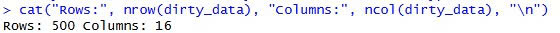
\includegraphics[width=0.8\linewidth]{Image/Chapter_3/hinh_1}
        \caption{Kết quá thể hiện số dòng và cột.}
        \label{Ket_qua_the_hien_so_dong_va_cot}
    \end{figure}

    Dữ liệu của một số dòng đầu tiên của dữ liệu:
    \begin{figure}[htbp]
        \centering
        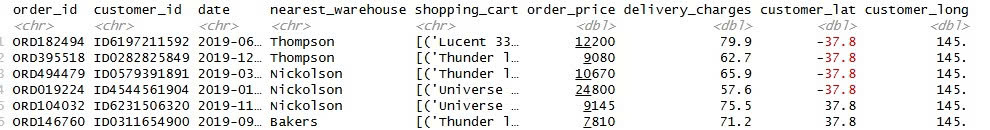
\includegraphics[width=1\linewidth]{Image/Chapter_3/hinh_2}
        \caption{Kết quá thể hiện các dòng đầu tiên.}
        \label{Ket_qua_the_hien_dong_dau_tien}
    \end{figure}

\subsection{Xác định các biến cần thiết}
    Sau khi xác định được các thông số đầu vào, ta cần giữ lại các biến cố định phụ vụ cho việc phân tích số liệu và thống kê.
    Ta sử dụng các tập lệnh (command):
    \begin{enumerate}
        \item c(): tạo vector chuỗi ký tự chứa danh sách các biến cần thiết.
        \item new\_df <- df[rows, columns]: trích xuất 1 phần dữ liệu từ df sang new\_df trong khoảng [rows] và [columns].
        \item names(): trích xuất các biến hiện có trong dữ liệu.
    \end{enumerate}

    \begin{lstlisting}
selected_vars <- c("nearest_warehouse", "delivery_charges", "coupon_discount", "order_total", "season", "is_expedited_delivery", "distance_to_nearest_warehouse", "is_happy_customer", "customer_lat", "customer_long", "order_price")
new_data <- dirty_data[, selected_vars]
cat("Rows:", nrow(new_data), "Columns:", ncol(new_data), "\n")
print(names(new_data))
    \end{lstlisting}

    Kết quả thu được: \\
    Dữ liệu mới sau khi xác định các biến cần thiết là: 500 dòng, 11 cột.
    \begin{figure}[htbp]
        \centering
        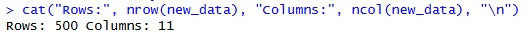
\includegraphics[width=0.8\linewidth]{Image/Chapter_3/hinh_3}
        \caption{Kết quá thể hiện các dòng và cột sau khi loại bỏ các biến.}
        \label{Ket_qua_the_hien_dong_va_cot_sau_khi_loai_bo_cac_bien}
    \end{figure}

    Từ đó, ta xác định được các biến cần thiết:
    \begin{figure}[htbp]
        \centering
        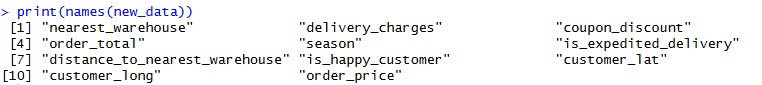
\includegraphics[width=1\linewidth]{Image/Chapter_3/hinh_4}
        \caption{Kết quá thể hiện tên các biến cần thiết.}
        \label{Ket_qua_the_hien_ten_cac_bien_can_thiet}
    \end{figure}

    Vì mục tiêu sau khi xử lý dữ liệu đầu vào được dùng để phân tích và thống kê liên quan đến phí giao hàng:
    \begin{itemize}
        \item[] \textbf{Các biến được loại bỏ:} các biến mang tính danh định và mang tính phân loại trong việc giao hàng: "order\_id", "customer\_id", "date", "shopping\_cart" và "date". 
        \item[] \textbf{Các biến cần được giữ lại:} nearest\_warehouse, delivery\_charges, coupon\_discount, order\_total, season, is\_expedited\_delivery, distance\_to\_nearest\_warehouse, is\_happy\_customer, customer\_lat, customer\_long, order\_price.
    \end{itemize}

\subsection{Kiểm tra thiếu dữ liệu, chuẩn hoá dữ liệu, kiểm tra công thức}
    Sau khi có được các dữ liệu cần thiết cho việc phân tích phí giao hàng (delivery charges), dữ liệu phải được kiểm tra và chỉnh sửa những lỗi như: biến thiếu dữ liệu, biến phụ thuộc công thức, dữ liệu dạng chuỗi (string) phải được chuẩn hoá định dạng.
    \subsubsection{Kiểm tra giá trị thiếu}
        Ta sử dụng các lệnh (command):
        \begin{enumerate}
            \item is.na(): kiểm tra dữ liệu đưa vào, trả về ma trận giá trị TRUE (nếu giá trị là NA (Not Available)) và FALSE (nếu có giá trị).
            \item apply(is.na(new\_data), 2, sum): tổng từng cột, trả về giá trị các ô có giá trị là NA.
            \item sapply(new\_data, function(x) if (is.character(x)) sum(trimws(x) == "", na.rm = TRUE) else 0): kiểm tra xem ô đó phải là chuỗi và "" hay " " không, đếm tất cả các ô chuỗi rỗng đó.
            \item for (col in names(new\_data)): duyệt qua từng cộng của new\_data.
            \item is.character(new\_data[[col]]): chỉ duyệt những cột có kiểu dữ liệu là dạng chuỗi (string).
            \item which(): tìm vị trí dòng của ô được duyệt đến.
            \item new\_data[[col]][empty\_index] <- NA: quy chuẩn các giá trị thiếu vào mục NA (Not Available).
        \end{enumerate}

        \begin{lstlisting}
missing_before <- apply(is.na(new_data), 2, sum)
empty_before <- sapply(new_data, function(x) if (is.character(x)) sum(trimws(x) == "", na.rm = TRUE) else 0)
print(missing_before)
print(empty_before)
for (col in names(new_data)) {
if (is.character(new_data[[col]])) {
    empty_index <- which(trimws(new_data[[col]]) == "")
    new_data[[col]][empty_index] <- NA
}
}
rows_before_missing <- nrow(new_data)
new_data <- na.omit(new_data)
cat("Rows removed:", rows_before_missing - nrow(new_data), "\n")
        \end{lstlisting}

        Kết quả thu được: \\
        Sau khi phân tích các lỗi thiếu, chuẩn hoá các dạng thiếu, khoảng trống thành dạng NA, ta loại bỏ được 0 dòng bị thiếu, điều này chứng tỏ rằng dữ liệu đầu vào có đủ dữ liệu cho từng biến.
        \begin{figure}[htbp]
            \centering
            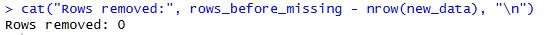
\includegraphics[width=0.8\linewidth]{Image/Chapter_3/hinh_5}
            \caption{Kết quá thể hiện 0 dòng được xoá.}
            \label{Ket_qua_the_hien_ten_0_dong_duoc_xoa}
        \end{figure}

        \subsubsection{Chuẩn hoá định dạng dữ liệu}
        Sau khi xử lý các giá trị bị thiếu, dữ liệu đầu vào vẫn còn các lỗi như thiếu đồng bộ giữa ký tự chuỗi hoa và ký tự chuỗi thường trong cột "nearest\_warehouse" và "season", thế nên, bộ dữ liệu cần được xử lý chuẩn hoá định dạng.\\
        Ta sử dụng các lệnh (command):
        \begin{enumerate}
            \item unique(): trích xuất ra giá trị phân biệt (không lặp lại) trong dữ liệu.
            \item trimws(): cắt bỏ các khoảng trắng thừa ở hai đầu chuỗi ký tự.
            \item tolower(): chuyển dạng chuỗi ký tự về dạng thường.
            \item unname(): loại bỏ nhãn tên, chỉ giữ lại chuỗi.
        \end{enumerate}

        \begin{lstlisting}
print(unique(new_data$nearest_warehouse))
print(unique(new_data$season))
warehouse_map <- c(thompson = "Thompson", nickolson = "Nickolson", bakers = "Bakers")
warehouse_key <- tolower(trimws(new_data$nearest_warehouse))
new_data$nearest_warehouse <- unname(warehouse_map[warehouse_key])
season_map <- c(spring = "Spring", summer = "Summer", autumn = "Autumn", winter = "Winter")
season_key <- tolower(trimws(new_data$season))
new_data$season <- unname(season_map[season_key])
print(table(new_data$nearest_warehouse))
print(table(new_data$season))
        \end{lstlisting}

        Kết quả thu được: \\
        Sau khi xử lý và trích xuất ký tự in hoa và in thường, ta được các kết quả như sau:
        \begin{figure}[htbp]
            \centering
            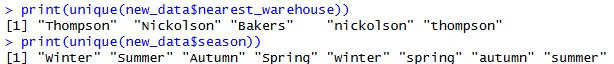
\includegraphics[width=0.8\linewidth]{Image/Chapter_3/hinh_6}
            \caption{Kết quá thể hiện các giá trị unique.}
            \label{Ket_qua_the_hien_ten_cac_gia_tri_unique}
        \end{figure}
        
        Sau khi đã chuẩn hoá các ký tự theo key, ta có thể đưa ra số liệu về tổng đơn hàng ở từng kho và từng mùa. 
        \begin{figure}[htbp]
            \centering
            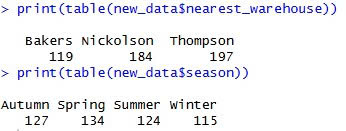
\includegraphics[width=0.6\linewidth]{Image/Chapter_3/hinh_7}
            \caption{Kết quá thể hiện số lần tên các kho hàng và mùa mua hàng.}
            \label{Ket_qua_the_hien_so_lan_ten_cac_kho_hang_va_mua_mua_hang}
        \end{figure}

    \subsubsection{Kiểm tra công thức tính tổng tiền và chỉnh sửa sai số}
        Sau khi đã xử lý các vấn đề về việc thống nhất định dạng dữ liệu, ta cần xử lý sự chính xác mối liên hệ giữa những biến trong dữ liệu. Trong đó, biến "order\_total" có mối liên hệ với các biến còn lại.

        Cụ thể, biến "order\_total" được tính như sau:
        \begin{equation*}
            \text{order\_total} = \text{order\_price} \times \left(1 - \frac{\text{coupon\_discount}}{100}\right) + \text{delivery\_charges}
            \label{eq:order_total}
        \end{equation*}

        \begin{lstlisting}
new_data$calculated_total <- new_data$order_price * (1 - new_data$coupon_discount / 100) + new_data$delivery_charges
mismatch_before <- sum(abs(new_data$order_total - new_data$calculated_total) > 0.01)
cat("Rows outside tolerance before correction:", mismatch_before, "\n")
new_data$order_total <- new_data$calculated_total
mismatch_after <- sum(abs(new_data$order_total - new_data$calculated_total) > 0.01)
cat("Rows outside tolerance after correction:", mismatch_after, "\n")
        \end{lstlisting}

        Kết quả thu được: \\
        Số lỗi (giá trị không khớp với công thức) trước khi sửa chữa:
        \begin{figure}[htbp]
            \centering
            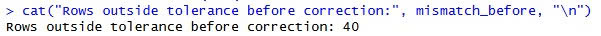
\includegraphics[width=0.8\linewidth]{Image/Chapter_3/hinh_8}
            \caption{Kết quá thể hiện số giá trị lệch.}
            \label{Ket_qua_the_hien_so_gia_tri_lech}
        \end{figure}

        Số lỗi sau khi đã áp dụng và đối sánh với lý thuyết công thức:
        \begin{figure}[htbp]
            \centering
            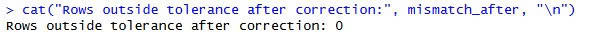
\includegraphics[width=0.8\linewidth]{Image/Chapter_3/hinh_9}
            \caption{Kết quá thể hiện số giá trị lệch sau khi sửa.}
            \label{Ket_qua_the_hien_so_gia_tri_lech_sau_khi_sua}
        \end{figure}
        
        Sau khi dữ liệu được xử lý và kiểm duyệt, ta có thể xoá cột "calculated\_total" (biến trung gian cho việc kiểm duyệt chính xác) và xuất đầu ra tập tin dữ liệu sạch "clean\_data\_full.csv"
        \begin{lstlisting}
new_data$calculated_total <- NULL
write_csv(new_data, "clean_data_full.csv")
        \end{lstlisting}

        
\section{Thống kê mô tả}

\subsection{Thống kê mô tả cho các biến định lượng}
    Đầu tiên, ta tiến hành tính các đại lượng thống kê mô tả cơ bản (Mean, Median, SD, Min, Max) cho các biến định lượng, với trọng tâm phân tích là biến chi phí giao hàng (delivery\_charges).
    Ta sử dụng các tập lệnh (command):
    \begin{enumerate}
        \item function(x): tự định nghĩa hàm để tính 5 thông số thống kê.
        \item apply(X, MARGIN, FUN): áp dụng hàm tính toán vừa tạo lên toàn bộ các cột dữ liệu định lượng.
    \end{enumerate}
    Phần code lập trình xử lý các thông số thống kê:

    \begin{lstlisting}
    clean_data <- read.csv("clean_data_full.csv")

    describe_function <- function(x) {
      c(Mean = mean(x, na.rm = TRUE),
        Median = median(x, na.rm = TRUE),
        SD = sd(x, na.rm = TRUE),
        Min = min(x, na.rm = TRUE),
        Max = max(x, na.rm = TRUE))
    }
    num_vars <- c("delivery_charges", "coupon_discount", "order_total", "distance_to_nearest_warehouse")
    des_table <- apply(clean_data[, num_vars], 2, describe_function)
    print(des_table)
    \end{lstlisting}
    \textbf{Kết quả thu được:}\\
    Bảng thống kê mô tả cho thấy chi tiết giá trị trung bình, trung vị, độ lệch chuẩn, giá trị lớn nhất và nhỏ nhất của chi phí giao hàng cùng các biến liên quan.
    \begin{figure}[htbp]
        \centering
        \fbox{\includegraphics[width=0.9\linewidth]{hinh_1.jpg} }
        \caption{Kết quả bảng thống kê mô tả các biến định lượng.}
        \label{Bang_thong_ke_mo_ta}
    \end{figure}\\
    Mặc dù trong clean\_data thì customer\_lat và customer\_long là hai biến định lượng, nhưng ta không đưa vào bảng để tính 5 thông số thống kê cơ bản (Mean, Median, SD, Min, Max) vì:\\
    
        \textbf{Ý nghĩa thống kê thực tiễn:} Việc tính trung bình (Mean) hay độ lệch chuẩn (SD) của vĩ độ và kinh độ khách hàng không mang lại bất kỳ ý nghĩa phân tích kinh tế hay logistics nào.\\
        
        \textbf{Vai trò riêng:} Các biến customer\_lat và customer\_long không dùng để tính toán các đại lượng đặc trưng trung tâm hay phân tán, mà chỉ được giữ lại chủ yếu để kiểm tra sự phân bố không gian và vẽ các biểu đồ (thường liên quan đến biến distance\_to\_nearest\_warehouse).  
\subsection{Thống kê số lượng cho các biến phân loại}
    Tiếp theo, ta lập bảng thống kê số lượng (tần số) để xem xét sự phân bố đơn hàng theo các biến định tính: mùa vụ (season), trạng thái giao hàng nhanh (is\_expedited\_delivery), kho hàng (nearest\_warehouse) và mức độ hài lòng của khách hàng (is\_happy\_customer).
    Ta sử dụng lệnh:
    \begin{enumerate}
        \item table(): lập bảng tần số đếm số lượng phần tử thuộc mỗi nhóm phân loại.
    \end{enumerate}

    \begin{lstlisting}
    freq_season <- table(clean_data$season)
    freq_expedited <- table(clean_data$is_expedited_delivery)
    freq_warehouse <- table(clean_data$nearest_warehouse)
    freq_happy <- table(clean_data$is_happy_customer)
    
    print(freq_season)
    print(freq_expedited)
    print(freq_warehouse)
    print(freq_happy)
    \end{lstlisting}
    \textbf{Kết quả thu được:}\\
    Dữ liệu số lượng được phân bổ cụ thể cho từng hạng mục:\\
    
    \textbf{Mùa:}
    \begin{figure}[H]
        \centering
        \fbox{\includegraphics[width=0.9\linewidth]{hinh_2.png}}
        \caption{Kết quả số lượng theo mùa.}
        \label{Bang_thong_ke_mo_ta}
    \end{figure}
    
    \textbf{Nhận xét:} Dữ liệu cho thấy sự phân bố đơn hàng giữa các mùa có sự khác biệt. Cao nhất là mùa Xuân với 134 đơn hàng, tiếp đó là mùa Thu với 127 đơn, mùa Hè với 124 đơn và thấp nhất là mùa Đông với 115 đơn hàng. Từ đó cho thấy mức độ tiêu thụ ở mùa Xuân tăng cao sớm, trong khi đó lại giảm đi ở mùa Đông.\\
    
    \textbf{Trạng thái giao hàng nhanh:}
    \begin{figure}[H]
        \centering
        \fbox{\includegraphics[width=0.3\linewidth]{hinh_3.png}}
        \caption{Kết quả số lượng theo trạng thái giao hàng nhanh.}
        \label{Bang_thong_ke_mo_ta}
    \end{figure}
    
    \textbf{Nhận xét:} Sự phân bố đơn hàng theo trạng thái giao hàng nhanh cho thấy có 249 đơn yêu cầu giao hàng nhanh (TRUE) và còn lại 251 đơn không yêu cầu giao hàng nhanh (FALSE). Từ đó cho thấy xu hướng người mua không yêu cầu giao hàng nhanh cao, nhưng so với người mua yêu cầu giao hàng nhanh thì tỉ lệ này khá cân bằng, khẳng định vai trò của dịch vụ giao hàng nhanh.\\
    
    \textbf{Kho gần nhất:}
    \begin{figure}[H]
        \centering
        \fbox{\includegraphics[width=0.9\linewidth]{hinh_4.png}}
        \caption{Kết quả số lượng theo kho gần nhất.}
        \label{Bang_thong_ke_mo_ta}
    \end{figure}
    
    \textbf{Nhận xét:} Dữ liệu cho thấy sự phân bố đơn hàng giữa giữa các kho không đồng đều. Trong đó ta thấy Thompson chiếm số lượng nhiều nhất là 197 đơn, tiếp đó là Nickolson là 184 đơn và thấp nhất là Bakers với 119 đơn hàng. Điều này chỉ ra rằng kho Thompson phổ biến hơn cũng như chất lượng dịch vụ tốt hơn so với 2 kho còn lại.\\

    \textbf{Mức độ hài lòng:}
    \begin{figure}[H]
        \centering
        \fbox{\includegraphics[width=0.3\linewidth]{hinh_5.png}}
        \caption{Kết quả số lượng theo mức độ hài lòng.}
        \label{Bang_thong_ke_mo_ta}
    \end{figure}
    
    \textbf{Nhận xét:} Dữ liệu cho thấy đa số các khách hàng đều có đánh giá tốt với 359 đơn hàng với mức độ hài lòng cao (TRUE), nhiều hơn 2,5 lần so với số đơn có mức độ hài lòng thấp (FALSE).\\
\subsection{Mô tả dữ liệu bằng đồ thị}
    Sau khi ta thực hiện phân tích, tổng hợp về số lượng đơn hàng theo các biến nearest\_warehouse, season, is\_expedited\_delivery và is\_happy\_customer, để trực quan hóa sự phân bố và các mối liên hệ liên quan đến chi phí giao hàng (delivery\_charges), ta tiến hành vẽ các đồ thị chuyên sâu.

    \subsubsection{Biểu đồ phân phối tần suất (Histogram)}
        Ta sử dụng lệnh \texttt{hist()} để vẽ biểu đồ phân phối.
        \begin{lstlisting}
    hist(clean_data$delivery_charges, main="Histogram of Delivery Charges", col="lightblue", xlab="Delivery Charges (USD)")
        \end{lstlisting}

        \begin{figure}[H]
            \centering
            \fbox{\includegraphics[width=0.8\linewidth]{do_thi_1.png}}
            \caption{Biểu đồ Histogram của chi phí giao hàng.}
            \label{Bieu_do_Histogram_Barplot}
        \end{figure}
        \textbf{Nhận xét:} Biểu đồ Histogram cho thấy phần lớn chi phí giao hàng tập trung ở mức giá trung bình, phân phối có dạng hơi lệch phải. Từ đó ta kết luận được phần lớn là các đơn hàng có phí thấp, một số ít là các đơn hàng có phí cao. 

    \subsubsection{Biểu đồ cột theo kho hàng (Barplot)}
        Mặc dù đồ thị Barplot giúp đếm số lượng đơn hàng theo kho, nhưng nó là nền tảng để giải thích yếu tố nearest\_warehouse - một biến độc lập sẽ được đưa vào mô hình hồi quy để dự báo deliver\_charges ở phần sau.
        \begin{lstlisting}
    barplot(freq_warehouse, main="Orders by Warehouse", col="lightgreen")
        \end{lstlisting}

        \begin{figure}[H]
            \centering
            \fbox{\includegraphics[width=0.8\linewidth]{do_thi_2.png}}
            \caption{Biểu đồ Barplot của số lượng đơn hàng tại các kho.}
            \label{Bieu_do_Barplot}
        \end{figure}
        \textbf{Nhận xét:} Biểu đồ cho thấy số lượng đơn hàng tại cả ba kho. Lần lượt là kho Baker với 119 đơn, tiếp đến là kho Nickolson với 184 đơn và kho Thompson với 197 đơn, cao nhất trong 3 kho. Từ đồ thị, ta nhân thấy rỏ nhất rằng số lượng đơn tập trung chủ yếu ở kho Thompson và Nickolson, trong khi đó số đơn tại kho Bakers lại ít hơn nhiều. Từ đó ta dể dàng so sánh mức độ phân bố đơn hàng tại các kho. 

    \subsubsection{Biểu đồ hộp theo mùa (Boxplot)}
        Để kiểm tra sự phân phối của biến delivery\_charge theo season, ta sử dụng biểu đồ hộp (Boxplot) bằng lệnh boxplot().
        \begin{lstlisting}
    boxplot(delivery_charges ~ season, data=clean_data, main="Delivery Charges by Season", col=c("pink","lightblue","lightgreen","yellow"), ylab="Delivery Charges")
        \end{lstlisting}

        \begin{figure}[H]
            \centering
            \fbox{\includegraphics[width=1\linewidth]{do_thi_3.png}}
            \caption{Biểu đồ Boxplot theo mùa.}
            \label{Bieu_do_Tuong_quan}
        \end{figure}
        \textbf{Nhận xét:} Từ biểu đồ Boxpot, ta nhận thấy rằng chi phí vận chuyển vào mùa xuân và mùa hè cao hơn 2 mùa còn lại là mùa thu và mùa đông. Từ đó ta dễ dàng nhận thấy yếu tố mùa có ảnh hưởng đến chi phí vận chuyển.

    \subsubsection{Biểu đồ hộp theo trạng thái giao hàng (Boxplot)}
        Biểu đồ Boxplot theo trạng thái giao hàng trực tiếp đối chiếu mức phí giao hàng giữa nhóm khách yêu cầu giao hàng nhanh (TRUE) và không yêu cầu giao hàng nhanh (FALSE).
        \begin{lstlisting}
    boxplot(delivery_charges ~ is_expedited_delivery, data=clean_data, main="Delivery Charges by Expedited Status", col=c("pink","lightblue"), ylab="Delivery Charges")
        \end{lstlisting}

        \begin{figure}[H]
            \centering
            \fbox{\includegraphics[width=0.8\linewidth]{do_thi_4.png}}
            \caption{Biểu đồ Boxplot theo trạng thái giao hàng.}
            \label{Bieu_do_QQ_Plot}
        \end{figure}
        \textbf{Nhận xét:} Dựa vào biểu đồ Boxpot theo trạng thái giao hàng, ta nhận thấy chi phí giao hàng khi khách yêu cầu giao hàng nhanh cao hơn nhiều so với chi phí giao hàng khi khách không yêu cầu giao hàng nhanh.

        \subsubsection{Đồ thị ma trận tương quan (Correlation Matrix)}
        Ma trận tương quan giúp tính toán mối liên hệ tuyến tính trực tiếp giữa delivery\_charges với khoảng cách (distance\_to\_nearest\_warehouse) và vị trí (ccustomer\_lat, customer\_long), nhằm loại trừ hiện tượng đa cộng tuyến trước khi xây dựng mô hình dự báo. Ta sử dụng thư viện Corrplot. 
        \begin{lstlisting}
    library(corrplot)
    cor_vars <- c("delivery_charges", "customer_lat", "customer_long", "distance_to_nearest_warehouse")
    cor_matrix <- cor(clean_data[, cor_vars])
    corrplot(cor_matrix, method="number")
        \end{lstlisting}

        \begin{figure}[H]
            \centering
            \fbox{\includegraphics[width=0.8\linewidth]{do_thi_5.png}}            \caption{Đồ thị ma trận tương quan (Correlation Matrix)}
            \label{Bieu_do_QQ_Plot}
        \end{figure}
        \textbf{Nhận xét:} Dựa vào đồ thị ma trận tương quan, ta nhận thấy được hệ số tương quan ứng với từng cặp biến độc lập gần bằng 0. Từ đó ta suy ra được các biến độc lập không có quan hệ tuyến tính với nhau, dẫn đến không xảy ra hiện tượng đa cộng tuyến.

        \subsubsection{Biểu đồ phân tán (Scatter Plot)}
        Biểu đồ phân tán thể hiện mối quan hệ tuyến tính giữa delivery\_charges với các biến distance\_to\_nearest\_warehouse, customer\_lat và customer\_long. Nó làm cơ sở cho mô hình hồi quy tuyến tính. 
        \begin{lstlisting}
    plot(clean_data$distance_to_nearest_warehouse, clean_data$delivery_charges,
     main = "Scatter Plot: Distance vs Delivery Charges",
     xlab = "Distance to Nearest Warehouse",
     ylab = "Delivery Charges",
     col = "darkred", pch = 16)
    plot(clean_data$customer_lat, clean_data$delivery_charges,
     main = "Scatter Plot: Customer lat vs Delivery Charges",
     xlab = "Customer lat ",
     ylab = "Delivery Charges ",
     col = "darkred", pch = 16)
    plot(clean_data$customer_long, clean_data$delivery_charges,
     main = "Scatter Plot: customer long vs Delivery Charges",
     xlab = "Customer long ",
     ylab = "Delivery Charges ",
     col = "darkred", pch = 16)
        \end{lstlisting}

        \begin{figure}[H]
            \centering
            \fbox{\includegraphics[width=0.7\linewidth]{do_thi_6.1.png}}
            \caption{Biểu đồ phân tán giữa Delivery Charge và Distance to Nearest Warehouse}
            \label{Bieu_do_QQ_Plot}
        \end{figure}

        \begin{figure}[H]
            \centering
            \fbox{\includegraphics[width=0.7\linewidth]{do_thi_6.2.png}}
            \caption{Biểu đồ phân tán giữa Delivery Charge và Customer lat}
            \label{Bieu_do_QQ_Plot}
        \end{figure}

        \begin{figure}[H]
            \centering
            \fbox{\includegraphics[width=0.7\linewidth]{do_thi_6.3.png}}
            \caption{Biểu đồ phân tán giữa Delivery Charge và Customer long}
            \label{Bieu_do_QQ_Plot}
        \end{figure}
        \textbf{Nhận xét:} Dựa vào 3 biểu đồ phân tán giữa delivery\_charges với customer\_lat, customer\_long và distance\_to\_nearest\_warehouse, ta nhận thấy các điểm dữa liệu phân bố không đồng đều hoặc tập trung thành từng cụm, không có một xu hướng tuyến tính rõ ràng. Điều này phù hợp với hệ số tương quan tương ứng với từng cặp biến độc lập gần bằng 0 như ở đồ thị ma trận tương quan. Chứng minh rằng khoảng cách hoặc tọa độ thông thường không có quan hệ tuyến tính với chi phí giao hàng.

        \subsubsection{Biểu đồ kiểm tra phân phối chuẩn (QQ-Plot)}
        Biểu đồ QQ-Plot kiểm tra trực tiếp xem biến delivery\_charges có tuân theo phân phối chuẩn hay không.
        \begin{lstlisting}
    qqnorm(clean_data$delivery_charges, 
       main = "Normal Q-Q Plot of Delivery Charges", 
       col = "black")
       qqline(clean_data$delivery_charges, col = "red", lwd = 2)
        \end{lstlisting}

        \begin{figure}[H]
            \centering
            \fbox{\includegraphics[width=0.8\linewidth]{do_thi_7.png}}
            \caption{Biểu đồ QQ-Plot kiểm tra phân phối chuẩn.}
            \label{Bieu_do_QQ_Plot}
        \end{figure}
        \textbf{Nhận xét:} Dựa vào đồ thị Normal Q-Q Plot, ta quan sát thấy các điểm dữ liệu phần lớn bám sát đường thẳng kỳ vọng chuẩn màu đỏ ở khu vực trung tâm. Tuy nhiên, ở hai khu vực phần đuôi (đặc biệt là đuôi phải), các quan trắc nằm lệch rõ rệt khỏi đường chuẩn. Điều này cho thấy phân phối của biến chi phí giao hàng có hiện tượng lệch và nhiều khả năng không tuân theo phân phối chuẩn một cách hoàn hảo.
\section{Thống kê suy diễn}
\textbf{Bối cảnh và mục tiêu của chương.} Trong thương mại điện tử, chi phí giao hàng là khoản khách hàng phải trả thêm ngoài giá hàng, đồng thời là yếu tố mà cửa hàng có thể điều chỉnh thông qua chính sách giá cước. Biết được chi phí giao hàng phụ thuộc vào những yếu tố nào (mùa vụ, loại hình giao hàng, kho xuất hàng, khoảng cách, mã giảm giá, \ldots) giúp cửa hàng định giá cước hợp lý và dự báo chi phí cho các đơn hàng mới. Vì vậy, trong chương này nhóm sử dụng các phương pháp thống kê suy diễn để đưa ra kết luận cho tổng thể toàn bộ đơn hàng của cửa hàng, nhằm trả lời ba câu hỏi nghiên cứu đã nêu ở phần kiến thức nền.

Nhóm sử dụng bộ dữ liệu \texttt{clean\_data\_full} gồm $n = 500$ đơn hàng (đã chuẩn hóa nhãn và tính lại \texttt{order\_total}, \textbf{chưa} loại ngoại lai của \texttt{order\_total}). Biến phụ thuộc chính là chi phí giao hàng \texttt{delivery\_charges} (USD), được giữ nguyên giá trị gốc. Riêng \texttt{order\_total} có phân phối lệch phải rất mạnh do 18 đơn hàng giá trị cực lớn (lớn nhất khoảng 853\,013 USD, trong khi trung vị chỉ khoảng 11\,294 USD); trong chương này biến đó chỉ tham gia với vai trò biến giải thích. Mức ý nghĩa được dùng xuyên suốt là $\alpha = 0.05$. Mỗi phương pháp dưới đây được trình bày theo bốn phần: \textbf{Mục tiêu}, \textbf{Kết quả}, \textbf{Nhận xét} và \textbf{Kết luận}; toàn bộ tính toán được thực hiện bằng R, đoạn mã và kết quả chạy được đặt trong phần Kết quả của từng mục.

\textbf{Mã R chuẩn bị dữ liệu (dùng cho toàn chương):}
\begin{lstlisting}
library(readr)
library(car)     
library(lmtest)  

dat <- read_csv("clean_data_full.csv", show_col_types = FALSE)
dat$season                <- factor(dat$season)            
dat$nearest_warehouse     <- factor(dat$nearest_warehouse) 
dat$is_expedited_delivery <- factor(dat$is_expedited_delivery, levels = c(FALSE, TRUE))
dat$is_happy_customer     <- factor(dat$is_happy_customer,     levels = c(FALSE, TRUE))
n <- nrow(dat); alpha <- 0.05
print(summary(dat$order_total))   
\end{lstlisting}
\textbf{Kết quả chạy:}
\begin{lstlisting}[style=rout]
    Min.  1st Qu.   Median     Mean  3rd Qu.     Max. 
   530.5   6388.3  11294.0  22564.6  17926.9 853012.7 
\end{lstlisting}

% ==========================================
\subsection{Ước lượng khoảng tin cậy}

\subsubsection{Khoảng tin cậy cho chi phí giao hàng trung bình}
\textbf{Mục tiêu:} Ước lượng khoảng tin cậy 95\% cho chi phí giao hàng trung bình $\mu$ của toàn bộ đơn hàng trong tổng thể. Do cỡ mẫu lớn ($n \ge 30$) và chưa biết $\sigma^2$, ta áp dụng công thức (9):
$$ \varepsilon = z_{\alpha/2}\frac{s}{\sqrt{n}}, \qquad \bar{x} - \varepsilon \le \mu \le \bar{x} + \varepsilon, \qquad \alpha = 0.05 \Longrightarrow z_{0.025} \approx 1.96. $$

\textbf{Kết quả:} Từ mẫu, $\bar{x} = 76.658$ USD, $s = 14.481$ USD, $n = 500$, suy ra sai số ước lượng $\varepsilon = 1.96 \times 14.481/\sqrt{500} \approx 1.27$ USD và
$$ \mu \in (75.389;\ 77.928) \text{ USD}. $$

\textbf{Mã R:}
\begin{lstlisting}
x <- dat$delivery_charges
me_z <- qnorm(0.975) * sd(x) / sqrt(n)       
cat("mean =", mean(x), " sd =", sd(x), " sai so =", me_z, "\n")
cat("CI (z):", mean(x) - me_z, "-", mean(x) + me_z, "\n")
\end{lstlisting}
\textbf{Kết quả chạy:}
\begin{lstlisting}[style=rout]
mean = 76.6582  sd = 14.48146  sai so = 1.269332 
CI (z): 75.38887 - 77.92753 
\end{lstlisting}

\textbf{Nhận xét:} Khoảng tin cậy khá hẹp (độ rộng khoảng 2.5 USD so với giá trung bình 76.66 USD), cho thấy với $n = 500$ trung bình mẫu ước lượng tương đối chính xác cho trung bình tổng thể.

\textbf{Kết luận:} Với độ tin cậy 95\%, ta có thể tin rằng chi phí giao hàng trung bình của mỗi đơn hàng tại cửa hàng nằm trong khoảng từ 75.389 USD đến 77.928 USD.

\subsubsection{Khoảng tin cậy cho tỷ lệ}
\textbf{Mục tiêu:} Ước lượng khoảng tin cậy 95\% cho tỷ lệ đơn hàng yêu cầu giao nhanh và tỷ lệ khách hàng hài lòng của tổng thể. Với mẫu lớn, ta áp dụng công thức (10):
$$ \varepsilon = z_{\alpha/2}\sqrt{\frac{\hat{p}(1-\hat{p})}{n}}, \qquad \hat{p} - \varepsilon \le p \le \hat{p} + \varepsilon, $$
với điều kiện xấp xỉ chuẩn $n\hat{p} \ge 5$ và $n(1-\hat{p}) \ge 5$.

\textbf{Kết quả:} Điều kiện xấp xỉ chuẩn thỏa mãn cho cả hai tỷ lệ (xem phần kết quả chạy). Kết quả được tổng hợp ở Bảng~\ref{tab:ci_tyle}.
\begin{table}[H]
    \centering
    \begin{tabular}{|l|c|c|c|}
    \hline
    \textbf{Tỷ lệ} & \textbf{Số đơn / $n$} & $\hat{p}$ & \textbf{KTC 95\%} \\ \hline
    Đơn giao hàng nhanh & 249 / 500 & 0.4980 & (0.4542; 0.5418) \\ \hline
    Khách hàng hài lòng & 359 / 500 & 0.7180 & (0.6786; 0.7574) \\ \hline
    \end{tabular}
    \caption{Khoảng tin cậy 95\% cho các tỷ lệ tổng thể}
    \label{tab:ci_tyle}
\end{table}

\textbf{Mã R:}
\begin{lstlisting}
for (v in c("is_expedited_delivery", "is_happy_customer")) {
  k <- sum(dat[[v]] == TRUE); p <- k / n
  e <- qnorm(0.975) * sqrt(p * (1 - p) / n)      
  cat(v, ": p =", round(p, 4), " CI =", round(p - e, 4), "-", round(p + e, 4),
      " (np =", k, ", n(1-p) =", n - k, ")\n")
}
\end{lstlisting}
\textbf{Kết quả chạy:}
\begin{lstlisting}[style=rout]
is_expedited_delivery : p = 0.498  CI = 0.4542 - 0.5418  (np = 249 , n(1-p) = 251 )
is_happy_customer : p = 0.718  CI = 0.6786 - 0.7574  (np = 359 , n(1-p) = 141 )
\end{lstlisting}

\textbf{Nhận xét:} Tỷ lệ giao nhanh trong mẫu xấp xỉ một nửa ($49.8\%$), còn tỷ lệ khách hàng hài lòng chiếm khoảng bảy phần mười ($71.8\%$).

\textbf{Kết luận:} Với độ tin cậy 95\%, trong tổng thể có khoảng $45.4\%$ đến $54.2\%$ đơn hàng yêu cầu giao nhanh và khoảng $67.9\%$ đến $75.7\%$ khách hàng hài lòng.

% ==========================================
\subsection{Kiểm định hai mẫu độc lập và phân tích tương quan}

\subsubsection{So sánh phí giao hàng giữa giao nhanh và giao thường}
\textbf{Mục tiêu:} Kiểm tra xem chi phí giao hàng trung bình của nhóm giao nhanh ($\mu_1$) có cao hơn nhóm giao thường ($\mu_2$) hay không. Hai mẫu độc lập và cỡ mẫu lớn ($n_1 = 249$, $n_2 = 251$, đều $\ge 30$) nên ta áp dụng kiểm định so sánh hai trung bình tổng thể theo công thức (11):
\begin{itemize}
    \item Giả thuyết kiểm định: $H_0: \mu_1 = \mu_2$ đối với $H_1: \mu_1 > \mu_2$.
    \item Thống kê kiểm định: $\displaystyle z_0 = \frac{\bar{x}_1 - \bar{x}_2}{\sqrt{\dfrac{s_1^2}{n_1} + \dfrac{s_2^2}{n_2}}}$.
    \item Quy tắc quyết định: với mức ý nghĩa $\alpha = 5\%$, ta bác bỏ $H_0$ nếu $p\text{-value} = P(Z > z_0) < \alpha$.
\end{itemize}

\textbf{Kết quả:} Từ mẫu, $\bar{x}_1 = 85.43$ USD, $s_1 = 13.61$ USD (giao nhanh) và $\bar{x}_2 = 67.96$ USD, $s_2 = 9.07$ USD (giao thường), do đó $z_0 = 16.868$ và $p\text{-value} \approx 3.9 \times 10^{-64}$.

\textbf{Mã R:}
\begin{lstlisting}
g1 <- dat$delivery_charges[dat$is_expedited_delivery == TRUE]
g0 <- dat$delivery_charges[dat$is_expedited_delivery == FALSE]
cat("mean:", mean(g1), mean(g0), " diff =", mean(g1) - mean(g0),
    " sd:", sd(g1), sd(g0), "\n")
z0 <- (mean(g1) - mean(g0)) / sqrt(var(g1)/length(g1) + var(g0)/length(g0)) 
cat("z0 =", z0, " p =", pnorm(z0, lower.tail = FALSE), "\n")
\end{lstlisting}
\textbf{Kết quả chạy:}
\begin{lstlisting}[style=rout]
mean: 85.42522 67.96104  diff = 17.46418  sd: 13.61355 9.068869 
z0 = 16.86784  p = 3.879417e-64 
\end{lstlisting}

\textbf{Nhận xét:} Giá trị $z_0 = 16.868$ rất lớn so với ngưỡng $1.645$ của kiểm định một phía mức $5\%$, và $p\text{-value}$ nhỏ hơn $\alpha$ rất nhiều. Chênh lệch trung bình mẫu giữa hai nhóm là $17.46$ USD, lớn hơn nhiều so với sai số chuẩn của hiệu hai trung bình.

\textbf{Kết luận:} Vì $p\text{-value} < \alpha = 0.05$, ta bác bỏ $H_0$. Với mức ý nghĩa 5\%, có đủ cơ sở thống kê để kết luận chi phí giao hàng của đơn giao nhanh cao hơn đơn giao thường.

\subsubsection{So sánh hai tỷ lệ theo mã giảm giá}
\textbf{Mục tiêu:} Kiểm tra xem việc đơn hàng có áp dụng mã giảm giá hay không có làm thay đổi tỷ lệ khách hàng hài lòng và tỷ lệ chọn giao nhanh hay không. Chia đơn hàng thành nhóm có mã giảm giá ($n_1 = 396$) và nhóm không có ($n_2 = 104$); ta áp dụng kiểm định so sánh hai tỷ lệ theo công thức (12):
\begin{itemize}
    \item Giả thuyết kiểm định: $H_0: p_1 = p_2$ đối với $H_1: p_1 \ne p_2$.
    \item Tỷ lệ mẫu gộp và thống kê kiểm định: $\displaystyle \hat{p}_c = \frac{x_1 + x_2}{n_1 + n_2}$, \quad $\displaystyle z_0 = \frac{\hat{p}_1 - \hat{p}_2}{\sqrt{\hat{p}_c(1-\hat{p}_c)\left(\dfrac{1}{n_1} + \dfrac{1}{n_2}\right)}}$.
    \item Quy tắc quyết định: bác bỏ $H_0$ nếu $p\text{-value} < \alpha = 5\%$.
\end{itemize}

\textbf{Kết quả:} Kết quả được tổng hợp ở Bảng~\ref{tab:hai_tyle}.
\begin{table}[H]
    \centering
    \begin{tabular}{|l|c|c|c|c|}
    \hline
    \textbf{Chỉ tiêu} & $\hat p_1$ (có mã) & $\hat p_2$ (không mã) & $z_0$ & $p\text{-value}$ \\ \hline
    Khách hàng hài lòng & 0.710 & 0.750 & $-0.815$ & 0.415 \\ \hline
    Chọn giao nhanh & 0.480 & 0.567 & $-1.588$ & 0.112 \\ \hline
    \end{tabular}
    \caption{Kiểm định hai tỷ lệ theo việc có/không có mã giảm giá}
    \label{tab:hai_tyle}
\end{table}

\textbf{Mã R:}
\begin{lstlisting}
dat$has_coupon <- dat$coupon_discount > 0
for (v in c("is_happy_customer", "is_expedited_delivery")) {
  tab <- table(dat$has_coupon, dat[[v]] == TRUE)
  print(tab)
  print(prop.test(c(tab["TRUE", "TRUE"], tab["FALSE", "TRUE"]),
                  c(sum(tab["TRUE", ]), sum(tab["FALSE", ])), correct = FALSE))
}
\end{lstlisting}
\textbf{Kết quả chạy:}
\begin{lstlisting}[style=rout]
 is_happy_customer 
       
        FALSE TRUE
  FALSE    26   78
  TRUE    115  281

	2-sample test for equality of proportions without continuity correction
X-squared = 0.6641, df = 1, p-value = 0.4151
alternative hypothesis: two.sided
95 percent confidence interval:
 -0.13487476  0.05406668
sample estimates:
  prop 1   prop 2 
0.709596 0.750000 

 is_expedited_delivery 
       
        FALSE TRUE
  FALSE    45   59
  TRUE    206  190

	2-sample test for equality of proportions without continuity correction
X-squared = 2.5231, df = 1, p-value = 0.1122
alternative hypothesis: two.sided
95 percent confidence interval:
 -0.19469247  0.01967304
sample estimates:
   prop 1    prop 2 
0.4797980 0.5673077 
\end{lstlisting}
(Khi \texttt{correct = FALSE}, thống kê \texttt{X-squared} của \texttt{prop.test} bằng $z_0^2$, nên $|z_0| = \sqrt{0.6641} = 0.815$ và $\sqrt{2.5231} = 1.588$; dấu âm vì $\hat p_1 < \hat p_2$.)

\textbf{Nhận xét:} Trong mẫu, nhóm không dùng mã giảm giá có tỷ lệ hài lòng và tỷ lệ chọn giao nhanh nhỉnh hơn một chút, nhưng chênh lệch ($4.0$ và $8.8$ điểm phần trăm) nhỏ so với dao động ngẫu nhiên, nhất là khi nhóm không có mã chỉ có $104$ đơn.

\textbf{Kết luận:} Cả hai $p\text{-value} > 0.05$ nên ta chưa đủ cơ sở bác bỏ $H_0$: chưa có bằng chứng cho thấy mã giảm giá làm thay đổi tỷ lệ khách hàng hài lòng hay tỷ lệ chọn giao nhanh.

\subsubsection{Tương quan giữa phí giao hàng và các biến định lượng}\label{sec:pearson}
\textbf{Mục tiêu:} Đánh giá mức độ liên hệ tuyến tính giữa chi phí giao hàng với khoảng cách đến kho gần nhất, tổng giá trị đơn hàng và mức chiết khấu. Ta tính hệ số tương quan mẫu Pearson $r$ theo công thức (7) và kiểm định theo công thức (8):
\begin{itemize}
    \item Giả thuyết kiểm định: $H_0: \rho = 0$ đối với $H_1: \rho \ne 0$.
    \item Thống kê kiểm định: $\displaystyle t_0 = \frac{r\sqrt{n-2}}{\sqrt{1-r^2}} \sim t(n-2)$.
    \item Quy tắc quyết định: bác bỏ $H_0$ nếu $p\text{-value} < \alpha = 5\%$.
\end{itemize}

\textbf{Kết quả:} Kết quả được tổng hợp ở Bảng~\ref{tab:pearson}.
\begin{table}[H]
    \centering
    \begin{tabular}{|l|c|c|}
    \hline
    \textbf{Biến} & \textbf{$r$ Pearson} & $p\text{-value}$ \\ \hline
    \texttt{distance\_to\_nearest\_warehouse} & $-0.053$ & 0.240 \\ \hline
    \texttt{order\_total} & $0.032$ & 0.475 \\ \hline
    \texttt{coupon\_discount} & $0.004$ & 0.929 \\ \hline
    \end{tabular}
    \caption{Hệ số tương quan mẫu giữa \texttt{delivery\_charges} và các biến định lượng}
    \label{tab:pearson}
\end{table}

\textbf{Mã R:}
\begin{lstlisting}
for (v in c("distance_to_nearest_warehouse", "order_total", "coupon_discount")) {
  ct <- cor.test(dat[[v]], dat$delivery_charges)
  cat(v, ": Pearson r =", round(ct$estimate, 4), " p =", round(ct$p.value, 4), "\n")
}
cat("So don co khoang cach > 10 km:", sum(dat$distance_to_nearest_warehouse > 10), "\n")
\end{lstlisting}
\textbf{Kết quả chạy:}
\begin{lstlisting}[style=rout]
distance_to_nearest_warehouse : Pearson r = -0.0527  p = 0.2399 
order_total : Pearson r = 0.032  p = 0.4752 
coupon_discount : Pearson r = 0.004  p = 0.9293 
So don co khoang cach > 10 km: 9 
\end{lstlisting}

\textbf{Nhận xét:} Cả ba hệ số $|r|$ đều rất gần $0$ (không quá $0.053$). Cần lưu ý \texttt{order\_total} và khoảng cách đều lệch phải mạnh (có $9$ đơn với khoảng cách lớn hơn $10$ km), nên hệ số Pearson của hai biến này chủ yếu phản ánh các đơn có giá trị cực đoan; vai trò của chúng được kiểm tra tiếp trong mô hình hồi quy (mục~\ref{sec:hoiquy}).

\textbf{Kết luận:} Mọi $p\text{-value} > 0.05$ nên ta chưa đủ cơ sở bác bỏ $H_0$: chưa có bằng chứng về tương quan tuyến tính giữa chi phí giao hàng và khoảng cách, tổng giá trị đơn hàng hay mức chiết khấu.

% ==========================================
\subsection{Phân tích phương sai 2 nhân tố (Two-Way ANOVA) và So sánh bội}\label{sec:anova}

\subsubsection{Mục tiêu và Đặt giả thuyết}
\textbf{Mục tiêu:} Đánh giá ảnh hưởng của mùa vụ (nhân tố $A$: Spring, Summer, Autumn, Winter, $a = 4$ mức), kho hàng gần nhất (nhân tố $B$: Bakers, Nickolson, Thompson, $b = 3$ mức) và hiệu ứng tương tác giữa chúng lên chi phí giao hàng. Mô hình ANOVA hai nhân tố có tương tác theo công thức (13):
$$ x_{ijk} = \mu + \alpha_i + \beta_j + (\alpha\beta)_{ij} + \varepsilon_{ijk}, \qquad \varepsilon_{ijk} \sim N(0, \sigma^2). $$
Ba cặp giả thuyết được kiểm định:
\begin{itemize}
    \item Hiệu ứng chính của mùa vụ: $H_0: \alpha_1 = \dots = \alpha_4 = 0$ đối với $H_1:$ tồn tại $i$ sao cho $\alpha_i \ne 0$ (tức $\mu_{Spring} = \mu_{Summer} = \mu_{Autumn} = \mu_{Winter}$ đối với có ít nhất một mùa khác biệt).
    \item Hiệu ứng chính của kho hàng: $H_0: \beta_1 = \beta_2 = \beta_3 = 0$ đối với $H_1:$ tồn tại $j$ sao cho $\beta_j \ne 0$ (tức $\mu_{Bakers} = \mu_{Nickolson} = \mu_{Thompson}$ đối với có ít nhất một kho khác biệt).
    \item Hiệu ứng tương tác: $H_0: (\alpha\beta)_{ij} = 0$ với mọi $i, j$ đối với $H_1:$ tồn tại $(i, j)$ sao cho $(\alpha\beta)_{ij} \ne 0$.
\end{itemize}
Quy tắc quyết định: với mỗi nguồn biến thiên, nếu $p\text{-value} < \alpha = 5\%$ thì bác bỏ $H_0$ tương ứng. Kết quả được đọc theo thứ tự: kiểm tra hiệu ứng tương tác trước, sau đó mới diễn giải các hiệu ứng chính.

\subsubsection{Kiểm tra giả định mô hình}
\textbf{Kết quả kiểm tra:} Ba giả định của mô hình ANOVA được kiểm tra như sau.
\begin{itemize}
    \item \textbf{Tính độc lập:} Mỗi dòng dữ liệu là một đơn hàng riêng biệt, không có quan sát lặp trên cùng một đối tượng; giả định được chấp nhận theo cách thu thập dữ liệu.
    \item \textbf{Phân phối chuẩn của phần dư (Shapiro-Wilk):} $W = 0.9907$, $p\text{-value} = 0.0031 < 0.05$. Đồ thị Q-Q Plot (Hình~\ref{fig:qq}) cho thấy các điểm bám sát đường chuẩn ở vùng giữa và chỉ lệch nhẹ ở hai đuôi.
    \item \textbf{Đồng nhất phương sai (Levene):} $F = 6.44$, $p\text{-value} = 5.1 \times 10^{-10} < 0.05$. Thiết kế cũng không cân bằng (cỡ ô từ 26 đến 52 đơn).
\end{itemize}

\begin{figure}[H]
    \centering
    \includegraphics[width=0.65\textwidth]{qqplot_anova.png}
    \caption{Đồ thị Q-Q Plot kiểm tra phân phối chuẩn của phần dư ANOVA}
    \label{fig:qq}
\end{figure}

\textbf{Mã R:}
\begin{lstlisting}
m_aov <- aov(delivery_charges ~ season * nearest_warehouse, data = dat)
print(table(dat$season, dat$nearest_warehouse))   
res <- resid(m_aov)
print(shapiro.test(res))
png("qqplot_anova.png")
qqnorm(res, main = "Q-Q Plot of ANOVA Residuals"); qqline(res, col = "red")
dev.off()
print(leveneTest(delivery_charges ~ season * nearest_warehouse, data = dat))
\end{lstlisting}
\textbf{Kết quả chạy:}
\begin{lstlisting}[style=rout]
        
         Bakers Nickolson Thompson
  Autumn     28        47       52
  Spring     35        48       51
  Summer     26        49       49
  Winter     30        40       45

	Shapiro-Wilk normality test
data:  res
W = 0.9907, p-value = 0.003062

Levene's Test for Homogeneity of Variance (center = median)
       Df F value    Pr(>F)    
group  11  6.4355 5.142e-10 ***
      488                      
\end{lstlisting}

\textbf{Nhận xét:} Hai giả định về phân phối chuẩn và đồng nhất phương sai không được thỏa mãn chặt chẽ ($p\text{-value} < 0.05$). Với $n = 500$, kiểm định Shapiro-Wilk rất nhạy với những lệch nhỏ khỏi phân phối chuẩn, và đồ thị Q-Q chỉ cho thấy lệch nhẹ ở hai đuôi.

\textbf{Kết luận:} Theo yêu cầu của giảng viên, khi các giả định không được thỏa mãn thì vẫn tiến hành phân tích. Nhóm ghi nhận các vi phạm trên và tiếp tục thực hiện ANOVA; các kết luận ở các mục sau cần được hiểu với lưu ý này.

\subsubsection{Kết quả phân tích ANOVA, Nhận xét và Kết luận}
\textbf{Kết quả:} Bảng ANOVA thu được từ R (Bảng~\ref{tab:anova}).
\begin{table}[H]
    \centering
    \begin{tabular}{|l|c|c|c|c|c|}
    \hline
    \textbf{Nguồn biến thiên} & \textbf{Df} & \textbf{Sum Sq} & \textbf{Mean Sq} & \textbf{F value} & \textbf{Pr($>$\textbf{F})} \\ \hline
    season & 3 & 27883 & 9294 & 59.679 & $<2 \times 10^{-16}$ *** \\ \hline
    nearest\_warehouse & 2 & 40 & 20 & 0.127 & 0.880 \\ \hline
    season:nearest\_warehouse & 6 & 722 & 120 & 0.773 & 0.591 \\ \hline
    Residuals & 488 & 76001 & 156 & & \\ \hline
    \end{tabular}
    \caption{Kết quả ANOVA 2 nhân tố}
    \label{tab:anova}
\end{table}

\begin{figure}[H]
    \centering
    \includegraphics[width=0.65\textwidth]{interaction_plot.png}
    \caption{Đồ thị tương tác giữa Mùa vụ và Kho hàng lên Chi phí giao hàng}
    \label{fig:int}
\end{figure}

\textbf{Mã R:}
\begin{lstlisting}
print(summary(m_aov))

png("interaction_plot.png")
interaction.plot(dat$season, dat$nearest_warehouse, dat$delivery_charges, fun = mean,
                 col = c("blue", "red", "green"), lty = 1, lwd = 2,
                 xlab = "Season", ylab = "Mean Delivery Charges", trace.label = "Warehouse")
dev.off()
\end{lstlisting}
\textbf{Kết quả chạy:}
\begin{lstlisting}[style=rout]
                          Df Sum Sq Mean Sq F value Pr(>F)    
season                     3  27883    9294  59.679 <2e-16 ***
nearest_warehouse          2     40      20   0.127  0.880    
season:nearest_warehouse   6    722     120   0.773  0.591    
Residuals                488  76001     156                   
\end{lstlisting}

\textbf{Nhận xét:} Theo quy tắc đọc kết quả, ta xét tương tác trước.
\begin{itemize}
    \item \textbf{Tương tác:} $Pr(>F) = 0.591 > 0.05$, chưa đủ cơ sở bác bỏ $H_0$. Các đường trong Hình~\ref{fig:int} có hình dạng tương tự nhau (cùng đạt đỉnh ở mùa Xuân và thấp nhất ở mùa Thu/Đông); chúng cắt nhau ở khoảng giữa mùa Xuân và mùa Hạ, nhưng chênh lệch giữa các kho trong cùng một mùa chỉ khoảng 1--4 USD, nhỏ so với độ lệch chuẩn khoảng 14.5 USD, phù hợp với kết quả kiểm định. Vì vậy có thể diễn giải các hiệu ứng chính.
    \item \textbf{Mùa vụ:} $Pr(>F) < 2 \times 10^{-16}$, bác bỏ $H_0$.
    \item \textbf{Kho hàng:} $Pr(>F) = 0.880 > 0.05$, chưa đủ cơ sở bác bỏ $H_0$.
\end{itemize}

\textbf{Kết luận:} Không có hiệu ứng tương tác giữa mùa vụ và kho hàng. Mùa vụ có tác động đến chi phí giao hàng, còn vị trí kho hàng không tạo ra sự khác biệt đáng kể về chi phí khi chỉ xét hai nhân tố này.

\subsubsection{So sánh bội (Tukey HSD)}
\textbf{Mục tiêu:} Do tương tác không có ý nghĩa, ta ước lượng lại mô hình cộng tính (chỉ gồm hai hiệu ứng chính) và dùng kiểm định hậu định Tukey HSD cho nhân tố có ý nghĩa và có từ 3 mức trở lên là \texttt{season}, nhằm chỉ ra cụ thể cặp mùa nào có chi phí trung bình khác nhau.

\textbf{Kết quả:} Trung bình mẫu theo mùa: Xuân $87.58$, Hạ $78.34$, Thu $69.78$, Đông $69.71$ USD. Kết quả so sánh từng cặp ở Bảng~\ref{tab:tukey}.
\begin{table}[H]
    \centering
    \begin{tabular}{|l|c|c|c|}
    \hline
    \textbf{Cặp mùa} & \textbf{Chênh lệch TB (USD)} & \textbf{KTC 95\%} & \textbf{$p$ adj} \\ \hline
    Xuân -- Thu & 17.80 & (13.82; 21.77) & $< 0.001$ \\ \hline
    Xuân -- Hạ  & 9.24  & (5.24; 13.24)  & $< 0.001$ \\ \hline
    Xuân -- Đông & 17.87 & (13.78; 21.95) & $< 0.001$ \\ \hline
    Hạ -- Thu   & 8.55  & (4.50; 12.61)  & $< 0.001$ \\ \hline
    Hạ -- Đông  & 8.63  & (4.47; 12.78)  & $< 0.001$ \\ \hline
    Đông -- Thu & $-0.07$ & ($-4.21$; 4.06) & 0.99997 \\ \hline
    \end{tabular}
    \caption{Tukey HSD theo mùa trên mô hình cộng tính (đầu ra \texttt{TukeyHSD(m\_add, \textquotedbl season\textquotedbl)})}
    \label{tab:tukey}
\end{table}

\textbf{Mã R:}
\begin{lstlisting}
m_add <- aov(delivery_charges ~ season + nearest_warehouse, data = dat)
print(summary(m_add))
print(TukeyHSD(m_add, "season"))     
\end{lstlisting}
\textbf{Kết quả chạy:}
\begin{lstlisting}[style=rout]
                   Df Sum Sq Mean Sq F value Pr(>F)    
season              3  27883    9294  59.844 <2e-16 ***
nearest_warehouse   2     40      20   0.128   0.88    
Residuals         494  76724     155                   

  Tukey multiple comparisons of means
    95% family-wise confidence level
Fit: aov(formula = delivery_charges ~ season + nearest_warehouse, data = dat)

$season
                      diff        lwr        upr     p adj
Spring-Autumn  17.79567752  13.817205  21.774150 0.0000000
Summer-Autumn   8.55381064   4.498030  12.609591 0.0000005
Winter-Autumn  -0.07199932  -4.207301   4.063303 0.9999675
Summer-Spring  -9.24186688 -13.244971  -5.238762 0.0000000
Winter-Spring -17.86767683 -21.951328 -13.784025 0.0000000
Winter-Summer  -8.62580996 -12.784816  -4.466804 0.0000008
\end{lstlisting}

\textbf{Nhận xét:} Năm trong sáu cặp mùa có $p\text{ adj} < 0.05$, riêng cặp Đông -- Thu có $p\text{ adj} = 0.99997$ (khoảng tin cậy chứa $0$). Chênh lệch lớn nhất là giữa mùa Xuân và hai mùa Thu, Đông (khoảng $17.8$ USD).

\textbf{Kết luận:} Chi phí giao hàng xếp theo thứ tự Xuân $>$ Hạ $>$ Thu $\approx$ Đông. Mùa Xuân đắt hơn mùa Thu khoảng 17.8 USD và đắt hơn mùa Hạ khoảng 9.2 USD; mùa Thu và mùa Đông không khác biệt có ý nghĩa thống kê. Vị trí kho không tạo chênh lệch phí.

% ==========================================
\subsection{Hồi quy tuyến tính đa biến (Multivariate Linear Regression)}\label{sec:hoiquy}

\subsubsection{Mục tiêu và Lựa chọn mô hình tối ưu}
\textbf{Mục tiêu:} Xây dựng phương trình dự báo chi phí giao hàng $Y$ dựa trên các biến: khoảng cách, tổng tiền, mã giảm giá, mùa vụ, kho hàng, giao hàng nhanh và mức độ hài lòng của khách hàng, theo mô hình (17):
$$ Y_i = \beta_0 + \beta_1 X_{i1} + \dots + \beta_p X_{ip} + \varepsilon_i, \qquad \varepsilon_i \sim N(0, \sigma^2). $$
Các biến phân loại được mã hóa thành biến giả: \texttt{season} (mức cơ sở Autumn), \texttt{nearest\_warehouse} (mức cơ sở Bakers), \texttt{is\_expedited\_delivery} và \texttt{is\_happy\_customer} (mức cơ sở FALSE); mô hình đầy đủ có 10 hệ số góc. Để loại bỏ các biến dư thừa, ta dùng phương pháp Stepwise hai chiều dựa trên việc cực tiểu hóa tiêu chuẩn AIC theo công thức (23). Với hệ số hồi quy $\beta_j$, ta kiểm định $H_0: \beta_j = 0$ đối với $H_1: \beta_j \ne 0$ bằng thống kê $t$ ở công thức (22), và kiểm định ý nghĩa tổng thể của mô hình bằng thống kê $F$ ở công thức (21); bác bỏ $H_0$ nếu $p\text{-value} < \alpha = 5\%$.

\textbf{Kết quả:} Thuật toán Stepwise loại \texttt{distance\_to\_nearest\_warehouse} ($p = 0.430$) và \texttt{order\_total} ($p = 0.316$) khỏi mô hình đầy đủ, giữ lại 5 biến: \texttt{coupon\_discount}, \texttt{season}, \texttt{nearest\_warehouse}, \texttt{is\_expedited\_delivery} và \texttt{is\_happy\_customer}; AIC giảm từ $3198.7$ xuống $3196.4$.

\textbf{Mã R:}
\begin{lstlisting}
lm_full <- lm(delivery_charges ~ distance_to_nearest_warehouse + order_total + coupon_discount +
                season + nearest_warehouse + is_expedited_delivery + is_happy_customer, data = dat)
print(summary(lm_full))
lm_opt <- step(lm_full, direction = "both", trace = 0)  
print(summary(lm_opt))
cat("AIC day du =", AIC(lm_full), " AIC toi uu =", AIC(lm_opt), "\n")
\end{lstlisting}
\textbf{Kết quả chạy:}
\begin{lstlisting}[style=rout]
--- lm_full ---
Coefficients:
                                Estimate Std. Error t value Pr(>|t|)    
(Intercept)                    5.112e+01  9.357e-01  54.627  < 2e-16 ***
distance_to_nearest_warehouse  2.369e-02  3.000e-02   0.790 0.430063    
order_total                   -3.524e-06  3.510e-06  -1.004 0.315862    
coupon_discount                5.735e-02  3.042e-02   1.885 0.059962 .  
seasonSpring                   1.756e+01  7.300e-01  24.055  < 2e-16 ***
seasonSummer                   1.050e+01  7.451e-01  14.094  < 2e-16 ***
seasonWinter                  -2.224e+00  7.582e-01  -2.934 0.003505 ** 
nearest_warehouseNickolson    -2.334e+00  6.919e-01  -3.373 0.000803 ***
nearest_warehouseThompson     -7.171e-01  6.825e-01  -1.051 0.293945    
is_expedited_deliveryTRUE      1.840e+01  5.276e-01  34.865  < 2e-16 ***
is_happy_customerTRUE          1.411e+01  5.878e-01  24.000  < 2e-16 ***
Residual standard error: 5.853 on 489 degrees of freedom
Multiple R-squared:  0.8399,	Adjusted R-squared:  0.8367 
F-statistic: 256.6 on 10 and 489 DF,  p-value: < 2.2e-16

--- lm_opt ---
lm(formula = delivery_charges ~ coupon_discount + season + nearest_warehouse + 
    is_expedited_delivery + is_happy_customer, data = dat)
Coefficients:
                           Estimate Std. Error t value Pr(>|t|)    
(Intercept)                51.23802    0.92042  55.668  < 2e-16 ***
coupon_discount             0.05596    0.03037   1.842 0.066014 .  
seasonSpring               17.49827    0.72534  24.124  < 2e-16 ***
seasonSummer               10.39791    0.74049  14.042  < 2e-16 ***
seasonWinter               -2.29359    0.75557  -3.036 0.002528 ** 
nearest_warehouseNickolson -2.33431    0.69097  -3.378 0.000787 ***
nearest_warehouseThompson  -0.76343    0.68132  -1.121 0.263040    
is_expedited_deliveryTRUE  18.36457    0.52679  34.861  < 2e-16 ***
is_happy_customerTRUE      14.04507    0.58559  23.984  < 2e-16 ***
Residual standard error: 5.851 on 491 degrees of freedom
Multiple R-squared:  0.8394,	Adjusted R-squared:  0.8368 
F-statistic: 320.8 on 8 and 491 DF,  p-value: < 2.2e-16

AIC day du = 3198.743  AIC toi uu = 3196.43 
\end{lstlisting}

\textbf{Nhận xét:} Stepwise chọn mô hình theo AIC chứ không theo $p\text{-value}$ của từng hệ số. Vì vậy \texttt{coupon\_discount} vẫn được giữ lại (AIC giảm nhẹ) dù hệ số không có ý nghĩa ở mức 5\% ($p = 0.066$); nhân tố \texttt{nearest\_warehouse} được giữ nguyên cả nhân tố vì hệ số của kho Nickolson có ý nghĩa ($p = 0.0008$) dù mức Thompson riêng lẻ không có ý nghĩa. Việc \texttt{distance\_to\_nearest\_warehouse} và \texttt{order\_total} bị loại nhất quán với kết quả tương quan ở mục~\ref{sec:pearson}.

\textbf{Kết luận:} Mô hình tối ưu theo AIC gồm 5 biến độc lập nêu trên; khoảng cách đến kho và tổng giá trị đơn hàng không giúp giải thích thêm chi phí giao hàng.

\subsubsection{Kiểm tra giả định mô hình}\label{sec:gdhq}
\textbf{Mục tiêu:} Kiểm tra các giả định của mô hình hồi quy trên mô hình cuối cùng (5 biến): tuyến tính và kỳ vọng sai số bằng 0, phương sai sai số đồng nhất, phân phối chuẩn của phần dư, không có đa cộng tuyến và không có điểm ảnh hưởng mạnh, theo mục 2.5.5 của kiến thức nền.

\textbf{Kết quả:} Các kết quả kiểm tra ở Hình~\ref{fig:diag} và phần kết quả chạy; mọi kiểm tra đều chạy trên \texttt{lm\_opt}.
\begin{itemize}
    \item \textbf{Tuyến tính và kỳ vọng sai số bằng 0:} Trong đồ thị Residuals vs Fitted (Hình~\ref{fig:diag}) đường làm trơn nằm gần $e_i = 0$, chỉ cong nhẹ.
    \item \textbf{Phương sai sai số đồng nhất:} Đồ thị Scale-Location không có hình phễu; kiểm định Breusch--Pagan cho $BP = 13.05$, $df = 8$, $p = 0.110 > 0.05$.
    \item \textbf{Phân phối chuẩn phần dư:} Shapiro--Wilk $W = 0.979$, $p = 1.28 \times 10^{-6} < 0.05$; Q-Q Plot cho thấy lệch chủ yếu ở hai đuôi.
    \item \textbf{Đa cộng tuyến:} VIF của \texttt{coupon\_discount}, \texttt{is\_expedited\_delivery}, \texttt{is\_happy\_customer} lần lượt là $1.006$, $1.013$, $1.014$; $GVIF^{1/(2\cdot df)}$ của \texttt{season} và \texttt{nearest\_warehouse} lần lượt là $1.004$ và $1.003$.
    \item \textbf{Điểm ảnh hưởng mạnh (Cook's Distance):} Với ngưỡng $D_i > 4/n$ có 29 quan sát vượt ngưỡng, giá trị lớn nhất là $D = 0.046$ (quan sát 468).
\end{itemize}

\begin{figure}[H]
    \centering
    \includegraphics[width=0.85\textwidth]{lm_diagnostics.png}
    \caption{Các biểu đồ chẩn đoán của mô hình hồi quy cuối cùng}
    \label{fig:diag}
\end{figure}

\textbf{Mã R:}
\begin{lstlisting}
print(vif(lm_opt))                    
print(shapiro.test(resid(lm_opt)))
print(bptest(lm_opt))                 
cd <- cooks.distance(lm_opt)
cat("Cook's D > 4/n:", sum(cd > 4 / n), " | max =", max(cd), " | dong:", which.max(cd), "\n")
png("lm_diagnostics.png", width = 800, height = 600)
par(mfrow = c(2, 2)); plot(lm_opt); par(mfrow = c(1, 1)); dev.off()
\end{lstlisting}
\textbf{Kết quả chạy:}
\begin{lstlisting}[style=rout]
                          GVIF Df GVIF^(1/(2*Df))
coupon_discount       1.005917  1        1.002954
season                1.022484  3        1.003713
nearest_warehouse     1.012268  2        1.003053
is_expedited_delivery 1.013326  1        1.006641
is_happy_customer     1.014163  1        1.007057

Shapiro-Wilk normality test
data:  resid(lm_opt)
W = 0.97897, p-value = 1.28e-06

studentized Breusch-Pagan test
data:  lm_opt
BP = 13.053, df = 8, p-value = 0.11

Cook's D > 4/n: 29  | max = 0.04579479  | dong: 468 
\end{lstlisting}

\textbf{Nhận xét:} Giả định tuyến tính, phương sai sai số đồng nhất và không đa cộng tuyến được thỏa mãn (các hệ số VIF đều gần $1$, rất nhỏ so với ngưỡng $5$). Phần dư không chuẩn tuyệt đối. Có 29 quan sát vượt ngưỡng $4/n$, nhưng giá trị $D$ lớn nhất chỉ là $0.046$, xa mức $1$, nên không có điểm nào ảnh hưởng nghiêm trọng đến các hệ số hồi quy.

\textbf{Kết luận:} Theo yêu cầu của giảng viên, khi một giả định (phân phối chuẩn của phần dư) không được thỏa mãn thì vẫn tiếp tục xây dựng hồi quy; với $n = 500$, các suy diễn về hệ số vẫn có thể xem là khá vững nhờ định lý giới hạn trung tâm.

\subsubsection{Phương trình hồi quy, Nhận xét và Kết luận}
\textbf{Kết quả:} Bảng hệ số của mô hình tối ưu (Bảng~\ref{tab:hq}) và phương trình hồi quy ước lượng.
\begin{table}[H]
    \centering
    \begin{tabular}{|l|c|c|c|c|}
    \hline
    \textbf{Biến} & \textbf{Estimate} & \textbf{Std. Error} & \textbf{t value} & \textbf{Pr($>|$\textbf{t}$|$)} \\ \hline
    (Intercept) & 51.2380 & 0.9204 & 55.668 & $< 2\times 10^{-16}$ *** \\ \hline
    coupon\_discount & 0.0560 & 0.0304 & 1.842 & 0.066 \\ \hline
    seasonSpring & 17.4983 & 0.7253 & 24.124 & $< 2\times 10^{-16}$ *** \\ \hline
    seasonSummer & 10.3979 & 0.7405 & 14.042 & $< 2\times 10^{-16}$ *** \\ \hline
    seasonWinter & $-2.2936$ & 0.7556 & $-3.036$ & 0.0025 ** \\ \hline
    nearest\_warehouseNickolson & $-2.3343$ & 0.6910 & $-3.378$ & 0.0008 *** \\ \hline
    nearest\_warehouseThompson & $-0.7634$ & 0.6813 & $-1.121$ & 0.263 \\ \hline
    is\_expedited\_deliveryTRUE & 18.3646 & 0.5268 & 34.861 & $< 2\times 10^{-16}$ *** \\ \hline
    is\_happy\_customerTRUE & 14.0451 & 0.5856 & 23.984 & $< 2\times 10^{-16}$ *** \\ \hline
    \end{tabular}
    \caption{Bảng hệ số hồi quy tuyến tính (Stepwise AIC)}
    \label{tab:hq}
\end{table}
\begin{align*}
\widehat{delivery} &= 51.24 + 0.06\cdot coupon + 17.50\cdot Spring + 10.40\cdot Summer - 2.29\cdot Winter \\
&\quad - 2.33\cdot Nickolson - 0.76\cdot Thompson + 18.36\cdot expedited + 14.05\cdot happy
\end{align*}
\textit{(Mức cơ sở: Mùa Thu, kho Bakers, các biến nhị phân bằng FALSE.)} Hệ số xác định $R^2 = 0.8394$, $R^2_{adj} = 0.8368$; sai số chuẩn phần dư $5.851$ USD (491 bậc tự do); kiểm định F tổng thể $F = 320.8$ ($df = 8;\ 491$), $p < 2.2 \times 10^{-16}$.

\textbf{Nhận xét:}
\begin{itemize}
    \item \textbf{Độ phù hợp:} Mô hình giải thích được $83.68\%$ biến thiên của chi phí giao hàng ($R^2_{adj}$); $p\text{-value}$ của kiểm định F nhỏ hơn $\alpha$ nên bác bỏ $H_0$, mô hình có ý nghĩa thống kê.
    \item \textbf{Giao hàng nhanh:} giữ nguyên các biến khác, chi phí tăng trung bình $18.36$ USD (tính chung cho các mùa).
    \item \textbf{Mùa vụ:} so với mùa Thu, chi phí cao hơn $17.50$ USD (Xuân), $10.40$ USD (Hạ) và thấp hơn $2.29$ USD (Đông).
    \item \textbf{Kho hàng:} kho Nickolson rẻ hơn kho Bakers khoảng $2.33$ USD; mức chênh nhỏ nhưng có ý nghĩa. Mức chênh này không xuất hiện trong ANOVA (mục~\ref{sec:anova}) vì khi chưa kiểm soát giao hàng nhanh và mức hài lòng, phương sai sai số còn rất lớn ($156$ so với $34$ ở mô hình này), làm che mờ hiệu ứng nhỏ.
    \item \textbf{Mã giảm giá:} hệ số không có ý nghĩa ở mức 5\% ($p = 0.066$); chưa đủ cơ sở cho rằng mã giảm giá ảnh hưởng đến chi phí giao hàng.
    \item \textbf{Mức hài lòng:} đơn có \texttt{is\_happy\_customer = TRUE} có chi phí cao hơn trung bình $14.05$ USD. Đây chỉ là mối liên hệ thống kê, không phải quan hệ nhân quả; hơn nữa mức hài lòng chỉ biết sau khi giao hàng nên biến này không dùng được để dự báo chi phí của đơn mới tại thời điểm đặt hàng (xem mục~\ref{sec:tt}).
\end{itemize}

\textbf{Kết luận:} Chi phí giao hàng phụ thuộc chủ yếu vào loại hình giao hàng (giao nhanh), mùa vụ (Xuân cao nhất) và kho xuất hàng (Nickolson thấp hơn Bakers); khoảng cách và tổng giá trị đơn hàng không ảnh hưởng đáng kể.

\subsubsection{Đánh giá hiệu năng dự báo (Train/Test 80-20)}\label{sec:tt}
\textbf{Mục tiêu:} Đánh giá khả năng dự báo trên dữ liệu mới của mô hình bằng cách chia ngẫu nhiên dữ liệu thành $80\%$ tập huấn luyện và $20\%$ tập kiểm tra, rồi tính MSE, RMSE, MAE theo các công thức (26)--(28) và hệ số $R^2_{test}$. Mô hình có RMSE, MAE càng nhỏ so với độ lệch chuẩn mẫu của \texttt{delivery\_charges} và $R^2_{test}$ càng cao thì dự báo càng chính xác. Nhóm so sánh hai mô hình: mô hình cuối (5 biến) và mô hình không dùng \texttt{is\_happy\_customer} (biến chỉ biết sau khi giao hàng).

\textbf{Kết quả:} Với \texttt{set.seed(42)}, tập huấn luyện gồm $400$ đơn và tập kiểm tra gồm $100$ đơn; kết quả ở Bảng~\ref{tab:tt42}. Để kết quả không phụ thuộc vào một lần chia, nhóm lặp $200$ lần chia ngẫu nhiên khác nhau (Bảng~\ref{tab:tt200}).
\begin{table}[H]
    \centering
    \small\setlength{\tabcolsep}{3pt}
    \begin{tabular}{|p{4.6cm}|c|c|c|c|}
    \hline
    \textbf{Mô hình} & \textbf{MSE} & \textbf{RMSE} & \textbf{MAE} & $R^2_{test}$ \\ \hline
    Mô hình cuối (5 biến) & 23.774 & 4.876 & 3.732 & 0.886 \\ \hline
    Mô hình không có \texttt{is\_happy\_customer} (\texttt{season} + \texttt{expedited}) & 59.465 & 7.711 & 6.150 & 0.715 \\ \hline
    \end{tabular}
    \caption{Hiệu năng dự báo trên tập kiểm tra (\texttt{set.seed(42)})}
    \label{tab:tt42}
\end{table}
\begin{table}[H]
    \centering
    \small\setlength{\tabcolsep}{3pt}
    \begin{tabular}{|p{4.6cm}|c|c|c|c|}
    \hline
    \textbf{Mô hình} & \textbf{MSE} & \textbf{RMSE} & \textbf{MAE} & $R^2_{test}$ \\ \hline
    Mô hình cuối (5 biến) & $34.32 \pm 5.93$ & $5.837 \pm 0.506$ & $4.367 \pm 0.366$ & $0.830 \pm 0.034$ \\ \hline
    Mô hình không có \texttt{is\_happy\_customer} & $74.68 \pm 9.17$ & $8.625 \pm 0.531$ & $6.847 \pm 0.444$ & $0.630 \pm 0.054$ \\ \hline
    \end{tabular}
    \caption{Trung bình $\pm$ độ lệch chuẩn của 200 lần chia ngẫu nhiên 80/20}
    \label{tab:tt200}
\end{table}

\textbf{Mã R:}
\begin{lstlisting}

lm_nohappy <- step(update(lm_full, . ~ . - is_happy_customer), direction = "both", trace = 0)
print(summary(lm_nohappy))

evaluate <- function(fml, seed = 42) {
  set.seed(seed)
  idx   <- sample(seq_len(n), size = floor(0.8 * n))
  train <- dat[idx, ]; test <- dat[-idx, ]
  fit   <- lm(fml, data = train)
  y <- test$delivery_charges; yhat <- predict(fit, test)
  c(MSE = mean((y - yhat)^2), RMSE = sqrt(mean((y - yhat)^2)), MAE = mean(abs(y - yhat)),
    R2_test = 1 - sum((y - yhat)^2) / sum((y - mean(y))^2))
}
res_tab <- rbind(`Mo hinh cuoi`   = evaluate(formula(lm_opt)),
                 `Khong co happy` = evaluate(formula(lm_nohappy)))
print(round(res_tab, 3))
cat("sd(delivery_charges) =", sd(dat$delivery_charges), "\n")

for (nm in c("Mo hinh cuoi", "Khong co happy")) {
  f <- switch(nm, `Mo hinh cuoi` = formula(lm_opt), `Khong co happy` = formula(lm_nohappy))
  rr <- sapply(1:200, function(s) evaluate(f, seed = s))
  print(round(cbind(mean = rowMeans(rr), sd = apply(rr, 1, sd)), 3))
}
\end{lstlisting}
\textbf{Kết quả chạy:}
\begin{lstlisting}[style=rout]
--- summary(lm_nohappy) ---
lm(formula = delivery_charges ~ season + is_expedited_delivery, data = dat)
Coefficients:
                          Estimate Std. Error t value Pr(>|t|)    
(Intercept)                61.1425     0.8496  71.970   <2e-16 ***
seasonSpring               17.3072     1.0664  16.230   <2e-16 ***
seasonSummer                9.3604     1.0875   8.608   <2e-16 ***
seasonWinter               -1.7560     1.1106  -1.581    0.114    
is_expedited_deliveryTRUE  17.9918     0.7738  23.252   <2e-16 ***
Residual standard error: 8.609 on 495 degrees of freedom
Multiple R-squared:  0.6494,	Adjusted R-squared:  0.6466 
F-statistic: 229.2 on 4 and 495 DF,  p-value: < 2.2e-16

--- print(round(res_tab, 3)) --- (set.seed(42))
                   MSE  RMSE   MAE R2_test
Mo hinh cuoi    23.774 4.876 3.732   0.886
Khong co happy  59.465 7.711 6.150   0.715
sd(delivery_charges) = 14.48146 

--- 200 lan chia ngau nhien: trung binh / do lech chuan ---
 Mo hinh cuoi
          mean    sd
MSE     34.323 5.934
RMSE     5.837 0.506
MAE      4.367 0.366
R2_test  0.830 0.034

 Khong co happy
          mean    sd
MSE     74.680 9.174
RMSE     8.625 0.531
MAE      6.847 0.444
R2_test  0.630 0.054
\end{lstlisting}

\textbf{Nhận xét:} Độ lệch chuẩn của chi phí giao hàng là $s = 14.48$ USD. Với \texttt{set.seed(42)}, RMSE của mô hình cuối là $4.876$ USD, chỉ bằng khoảng $34\%$ giá trị này, và $R^2_{test} = 0.886$ cao hơn $R^2$ trên toàn mẫu ($0.839$). Tuy nhiên lần chia này khá thuận lợi: kết quả của \texttt{set.seed(42)} cách mức trung bình khoảng $2$ độ lệch chuẩn (RMSE: $4.876$ so với $5.837 \pm 0.506$). Theo trung bình $200$ lần chia, RMSE là $5.84$ USD (khoảng $40\%$ độ lệch chuẩn) và $R^2_{test} \approx 0.83$, rất gần $R^2$ trên toàn mẫu, nên số liệu trung bình $200$ lần chia đáng tin cậy hơn để báo cáo. Khi bỏ \texttt{is\_happy\_customer}, $R^2_{test}$ giảm từ khoảng $0.83$ xuống khoảng $0.63$ và RMSE tăng từ $5.84$ lên $8.63$ USD.

\textbf{Kết luận:} Mô hình cuối giảm đáng kể sai số so với việc dự báo bằng trung bình và không có dấu hiệu quá khớp. Tuy nhiên vì mức hài lòng chưa biết tại thời điểm đặt hàng, mô hình thực sự dùng được để dự báo chi phí cho đơn hàng mới là mô hình không có \texttt{is\_happy\_customer} (gồm \texttt{season} và \texttt{is\_expedited\_delivery}), với $R^2_{test} \approx 0.63$ và RMSE khoảng $8.6$ USD.


\section{Thảo luận và mở rộng}

\subsection{Tổng kết kết quả chính}
Đề tài khảo sát các yếu tố ảnh hưởng đến phí giao hàng của cửa hàng bằng ba nhóm phương pháp: ước lượng và kiểm định giả thuyết, phân tích phương sai hai nhân tố kèm so sánh bội, và hồi quy tuyến tính bội. Các kết quả chính:
\begin{itemize}
    \item Phí giao hàng chịu ảnh hưởng rõ rệt của mùa vụ và hình thức giao hàng trong đó giao nhanh có phí cao hơn khoảng $18$ USD.
    \item Khoảng cách, giá trị đơn hàng và mã giảm giá không có tác động đáng kể và kho hàng chỉ có tác động nhỏ.
    \item Mô hình hồi quy giải thích khoảng $84\%$ biến thiên của phí giao hàng. Tuy nhiên mô hình này dùng cả mức độ hài lòng của khách , khi chỉ dùng các biến biết trước lúc đặt hàng thì khả năng dự báo đạt khoảng $63\%$.
\end{itemize}
Qua đó thấy được cửa hàng có thể định giá cước theo mùa vụ và hình thức giao hàng, thay vì theo khoảng cách hay giá trị đơn hàng.

\subsection{Ưu điểm và hạn chế của các phương pháp}
\begin{table}[H]
\centering
\setlength{\tabcolsep}{5pt}
\renewcommand{\arraystretch}{1.25}
\begin{tabular}{|p{2.8cm}|p{6.4cm}|p{6.4cm}|}
\hline
\textbf{Phương pháp} & \textbf{Ưu điểm} & \textbf{Hạn chế} \tabularnewline \hline
\raggedright\textbf{Ước lượng và kiểm định giả thuyết} \newline (khoảng tin cậy, kiểm định hai mẫu, tương quan Pearson) &
\raggedright\begin{itemize}[nosep,leftmargin=*]
    \item Đơn giản, dễ thực hiện và dễ diễn giải.
    \item Cho biết khoảng giá trị hợp lý của tham số và mức ý nghĩa thống kê của sự khác biệt.
    \item Phù hợp để kiểm tra nhanh một giả thuyết cụ thể.
    \item Hệ số tương quan cho biết nhanh mức độ liên hệ giữa hai biến định lượng.
\end{itemize} &
\raggedright\begin{itemize}[nosep,leftmargin=*]
    \item Cần cỡ mẫu đủ lớn hoặc phân phối gần chuẩn.
    \item Mỗi lần chỉ xét một biến hoặc hai nhóm; làm nhiều kiểm định riêng lẻ dễ tích lũy sai lầm loại I.
    \item Chỉ trả lời có khác biệt hay không, không mô hình hóa mối quan hệ giữa các biến.
    \item Hệ số tương quan Pearson chỉ đo quan hệ tuyến tính và nhạy với giá trị ngoại lai.
\end{itemize} \tabularnewline \hline
\raggedright\textbf{ANOVA hai nhân tố và so sánh bội (Tukey)} &
\raggedright\begin{itemize}[nosep,leftmargin=*]
    \item Dễ hiểu, so sánh trung bình giữa nhiều nhóm cùng lúc.
    \item Xét được đồng thời nhiều nhân tố và tương tác giữa chúng.
    \item Kết hợp so sánh bội cho biết nhóm nào khác nhau mà vẫn kiểm soát sai lầm loại I.
\end{itemize} &
\raggedright\begin{itemize}[nosep,leftmargin=*]
    \item Đòi hỏi giả định: phần dư chuẩn, phương sai đồng nhất, quan sát độc lập, nếu vi phạm thì kết luận kém tin cậy.
    \item Chỉ so sánh trung bình giữa các nhóm, không xây dựng được mô hình dự báo.
    \item Không đo được ảnh hưởng của các biến liên tục.
\end{itemize} \tabularnewline \hline
\raggedright\textbf{Hồi quy tuyến tính bội và Stepwise} &
\raggedright\begin{itemize}[nosep,leftmargin=*]
    \item Lượng hóa tác động của từng yếu tố khi giữ các yếu tố khác cố định, hệ số dễ diễn giải.
    \item Đánh giá được nhiều biến (liên tục và phân loại) cùng lúc.
    \item Dùng được để dự báo, Stepwise tự động lọc biến, giúp mô hình gọn hơn.
\end{itemize} &
\raggedright\begin{itemize}[nosep,leftmargin=*]
    \item Giả định mạnh: quan hệ tuyến tính, phần dư chuẩn, phương sai đồng nhất, không đa cộng tuyến.
    \item Nhạy với quan sát ngoại lai và điểm ảnh hưởng.
    \item Stepwise chọn biến theo tiêu chí thống kê (AIC) chứ không theo ý nghĩa nghiệp vụ.
    \item Hệ số chỉ phản ánh mối liên hệ, không chứng minh quan hệ nhân quả.
\end{itemize} \tabularnewline \hline
\end{tabular}
\caption{Ưu điểm và hạn chế của các phương pháp đã sử dụng}
\label{tab:uu_nhuoc}
\end{table}

\textbf{Vai trò và cách kết hợp các phương pháp.} Mỗi phương pháp đảm nhận một vai trò riêng, và trong đề tài nhóm đã kết hợp chúng theo ba bước:
\begin{itemize}
    \item \textbf{Bước 1 -- Sàng lọc yếu tố:} dùng ước lượng, kiểm định và ANOVA để xem yếu tố nào thật sự ảnh hưởng đến phí giao hàng. Kết quả cho thấy mùa vụ và hình thức giao hàng có ảnh hưởng, còn mã giảm giá và khoảng cách thì không rõ rệt.
    \item \textbf{Bước 2 -- Chọn biến:} dùng Stepwise để loại các biến thừa (khoảng cách, giá trị đơn hàng) và giúp giữ cho mô hình gọn.
    \item \textbf{Bước 3 -- Lượng hóa và dự báo:} dùng hồi quy tuyến tính bội trên các biến đã chọn để đo mức tác động ($R^2_{adj} \approx 0.84$) và dự báo phí giao hàng.
\end{itemize}

\textbf{Đánh giá chung.} Cách kết hợp này cho kết quả nhất quán giữa các phương pháp, nhưng mỗi phương pháp chỉ đáng tin khi các giả định của nó được kiểm tra. Trong đề tài, ANOVA vi phạm cả giả định phần dư chuẩn và phương sai đồng nhất, còn hồi quy chỉ vi phạm giả định phần dư chuẩn với phương sai đồng nhất vẫn thỏa mãn. Cùng với việc dữ liệu chỉ gồm $500$ đơn hàng trong một năm, các kết quả nên được xem là mối liên hệ thống kê mang tính tham khảo, cần kiểm chứng thêm trên dữ liệu rộng hơn.

\subsection{Đề xuất mở rộng}
\begin{itemize}
    \item Xét ANOVA hai nhân tố giữa mùa vụ và loại hình giao hàng (\texttt{is\_\allowbreak expedited\_\allowbreak delivery}), đồng thời thêm tương tác giao nhanh $\times$ mùa vào mô hình hồi quy, vì giao nhanh là yếu tố có tác động lớn nhất.
    \item Khi phần dư không chuẩn, có thể biến đổi biến phụ thuộc (ví dụ lấy logarit) hoặc dùng kiểm định phi tham số như Kruskal--Wallis; khi phương sai không đồng nhất, có thể dùng Welch's ANOVA (cho một nhân tố) hoặc ước lượng sai số chuẩn vững.
    \item Thử các mô hình học máy như Decision Tree, Random Forest hoặc Gradient Boosting: các mô hình này không giả định tuyến tính, nắm bắt được quan hệ phi tuyến và tương tác giữa các biến, xử lý biến phân loại tốt, và cho biết độ quan trọng của từng biến
    \item Mở rộng dữ liệu theo nhiều năm hoặc nhiều cửa hàng để kiểm tra tính ổn định của kết quả.
\end{itemize}
\section{Nguồn dữ liệu và nguồn code}

\subsection{Nguồn dữ liệu}
\begin{itemize}
    \item \textbf{Bộ dữ liệu:} \textit{Transactional Retail Dataset of Electronics Store} (tác giả Muhammad Shahrayar, đăng trên Kaggle).
    \item \textbf{Tệp sử dụng:} \texttt{dirty\_data.csv} (dữ liệu thô, gồm $500$ đơn hàng và $16$ biến).
    \item \textbf{Đường dẫn:}
\end{itemize}
\begin{center}
\url{https://www.kaggle.com/datasets/muhammadshahrayar/transactional-retail-dataset-of-electronics-store}
\end{center}
Dữ liệu sau khi làm sạch ở Chương 3 được lưu thành tệp \texttt{clean\_data\_full.csv} (giữ nguyên $500$ đơn hàng, không loại ngoại lai) và được dùng cho các phân tích ở Chương 4 và Chương 5.

\subsection{Nguồn code}
\begin{itemize}
    \item \textbf{Ngôn ngữ:} R (phần mềm RStudio).
    \item \textbf{Các gói R:} \texttt{readr}, \texttt{car}, \texttt{lmtest}, \texttt{corrplot}.
    \item \textbf{Mã nguồn:} \href{https://github.com/anhnguyenms2510421-design/BTL-XSTK/blob/main/Source_code/Source_code.r}{Mã nguồn ngôn ngữ R}  \\
    (\url{https://github.com/anhnguyenms2510421-design/BTL-XSTK/blob/main/Source_code/Source_code.r})
\end{itemize}


\nocite{*}
\printbibliography[title={TÀI LIỆU THAM KHẢO}]

\end{document}